\documentclass[../../AdvancementSummary.tex]{subfiles}

\begin{document}



%%%%%%%%%%%%%%%%%%%%%%%%%%%%%%%%%%%%%%%%%%%%%%%%%%%
\section{Role of the surface on tether-tether reactions within a signaling cluster}
%%%%%%%%%%%%%%%%%%%%%%%%%%%%%%%%%%%%%%%%%%%%%%%%%%%

\subsection{Introduction}
\subsubsection{Tethering}

Disordered proteins aid many reactions by acting as biological tethers. They may be permanent tethers tying two globular domains together or a domain to a surface (EXAMPLE, EXAMPLE, CITE, CITE). They may also be transient tethers, catching diffusing particles and tethering them to another molecule, i.e. formin \cite{Bryant2017}. By tethering molecules or surfaces together, disordered domains effectively increase the local concentration of a particle. This increases reaction rates by improving the probability of two molecules bumping into each other through restriction of their diffusive domain.

Given that a surface reduces the exploration space of a molecule, it will naturally increase the local concentration without a tether. However, it will also reduce the accessibility of a molecule by sometimes occluding, for example, an enzymatic domain from reaching its substrate in the correct orientation. Given that the surface has both positive and negative effects on reaction rates, how does being tethered to a surface impact a reaction compared to being tethered to a smaller domain? 

This type of interaction arises frequently with clustered reactions. For instance, the phosphorylation of a membrane tethered disordered domain by a membrane bound kinase (CITE). Experimental studies of such reactions are more easily performed on a sparse matrix such as dextran than on a hard surface. Therefore, it is important to understand the effect tethering to a surface has over tethering to a matrix. We explore how the presence of a surface influences the reach of a tethered domain and the overall local concentration.

\subsubsection{SHP-1}

%%%%%%%%%%%%%%%%%%%%%%%%%%%%%%%%%%%%%%%%%%%%%%%%%%%%%%%%%%%%%%%%%%%%%%%%%%%%%%%%%%%%%%%%%%%%%%%%%%%%%
%%%%%%%%%%%%%%%%%%%%%%%%%%%%%%%%%%%%%%%%%%%%%%%%%%%%%%%%%%%%%%%%%%%%%%%%%%%%%%%%%%%%%%%%%%%%%%%%%%%%%
\subsection{Model and Methods}

We first investigate the effects of a surface on a single tether without a bound ligand in free-space and half-space. We model the tether as a freely-jointed chain and the unbound ligand as an idealized ghost sphere located tangential to a single segment. To explore the effects of a surface on a single tether, we vary the number of segments and the size of the incoming ligand. We calculate quasi-equilibrium statistics for the FJC and unbound ligand in both free-space and half-space. We calculate how often a ligand is able to bind to an oriented sphere tangentially attached to the polymer, where `able to bind' refers to the specified sphere being empty of both other polymer segments and the surface. 

We next explore the effects of a surface on three specific tethers: PD-1, PEG-3, and PEG-28. PEG-3 and PEG-28 are tethers created by attaching a single immunoreceptor tyrosine inhibitory motif (ITIM) to a series of PEG linkers. Each tether is modeled as a freely-jointed chain characterized by their lengths as measured in Kuhn lengths. The tethers are made up of PEG linkers and amino acids, each of which contributes approximately 0.3nm to the length. We assume maximal flexibility in our model by assigning a Kuhn length,$\delta$, of 0.3nm. The contour lengths of each tether may be approximated as $N$ Kuhn lengths, where $N$ is the total number of PEG linkers and amino acids. Note that we consider the size of biotin to be negligible for our simulation. (Table \ref{table: Tethers})

%% Table of Tethers
\begin{table}
\caption{Structure and number of simulated segments in each explored tether. \label{table: Tethers}}
\begin{center}
\begin{tabular}{| c | p{10cm} | c |}
    \hline
        Tether Name & Structure & N \\ 
        \hline 
        PD-1    &   (37392 B2) Bio-SRAARGTIGARRTGQPLKEDPSAVPVFSV
                    DYGELDFQWREKTPEPPVPSVPEQTEY*ATIVFPSG            &   64   \\
        PEG-3   &   Bio-(PEG)3-DLQEVTY*IQLDHH                           &   16   \\ 
        PEG-28  &   Bio-(PEG)28-DLQEVTY*IQLDHH                          &   41   \\
    \hline
\end{tabular}
\end{center}
\end{table}

We investigate SHP-1 as a ligand bound to a tether. In order to simulate SHP-1 as a simple sphere, we estimate its size using three different assumptions. We first estimate the volume of SHP-1 based on its molecular weight, 67561Da,  as listed in UniProt entry P29350, assuming an average protein density of 1.41$g/cm^3$. \cite{Fischer2004}

%\cite{UniProtSHP1} 
%\cite{FischerProteinSci2004}

\begin{equation*}
(67.5 \times 1000 \mbox{Da}) * (1.66\times10^{-27} \mbox{kg / Da}) * (1000 \mbox{g / kg}) / (1.41 \mbox{g / cm}^3) = 79.468 \nm^3.
\end{equation*}

Approximating the phosphatase domain as a sphere, we can estimate a radius: 

\begin{align*}
V &= \frac{4}{3}\pi r^3 \\
79.468 \nm^3 &= \frac{4}{3} \pi r^3 \\
r &\approx 2.7 \nm \\
\end{align*}

For comparison, we also estimate an upper bound on the radius of SHP-1 from PyMol measurements of the SHP-1 structure (PDB 3PS5). Rounding up for measurement error, the longest part of the structure is 86 \AA. (Fig. \ref{fig: SHP1Diag}) From this we calculate a maximum radius of 4.3$nm$.

\begin{figure}[H]
\begin{center}
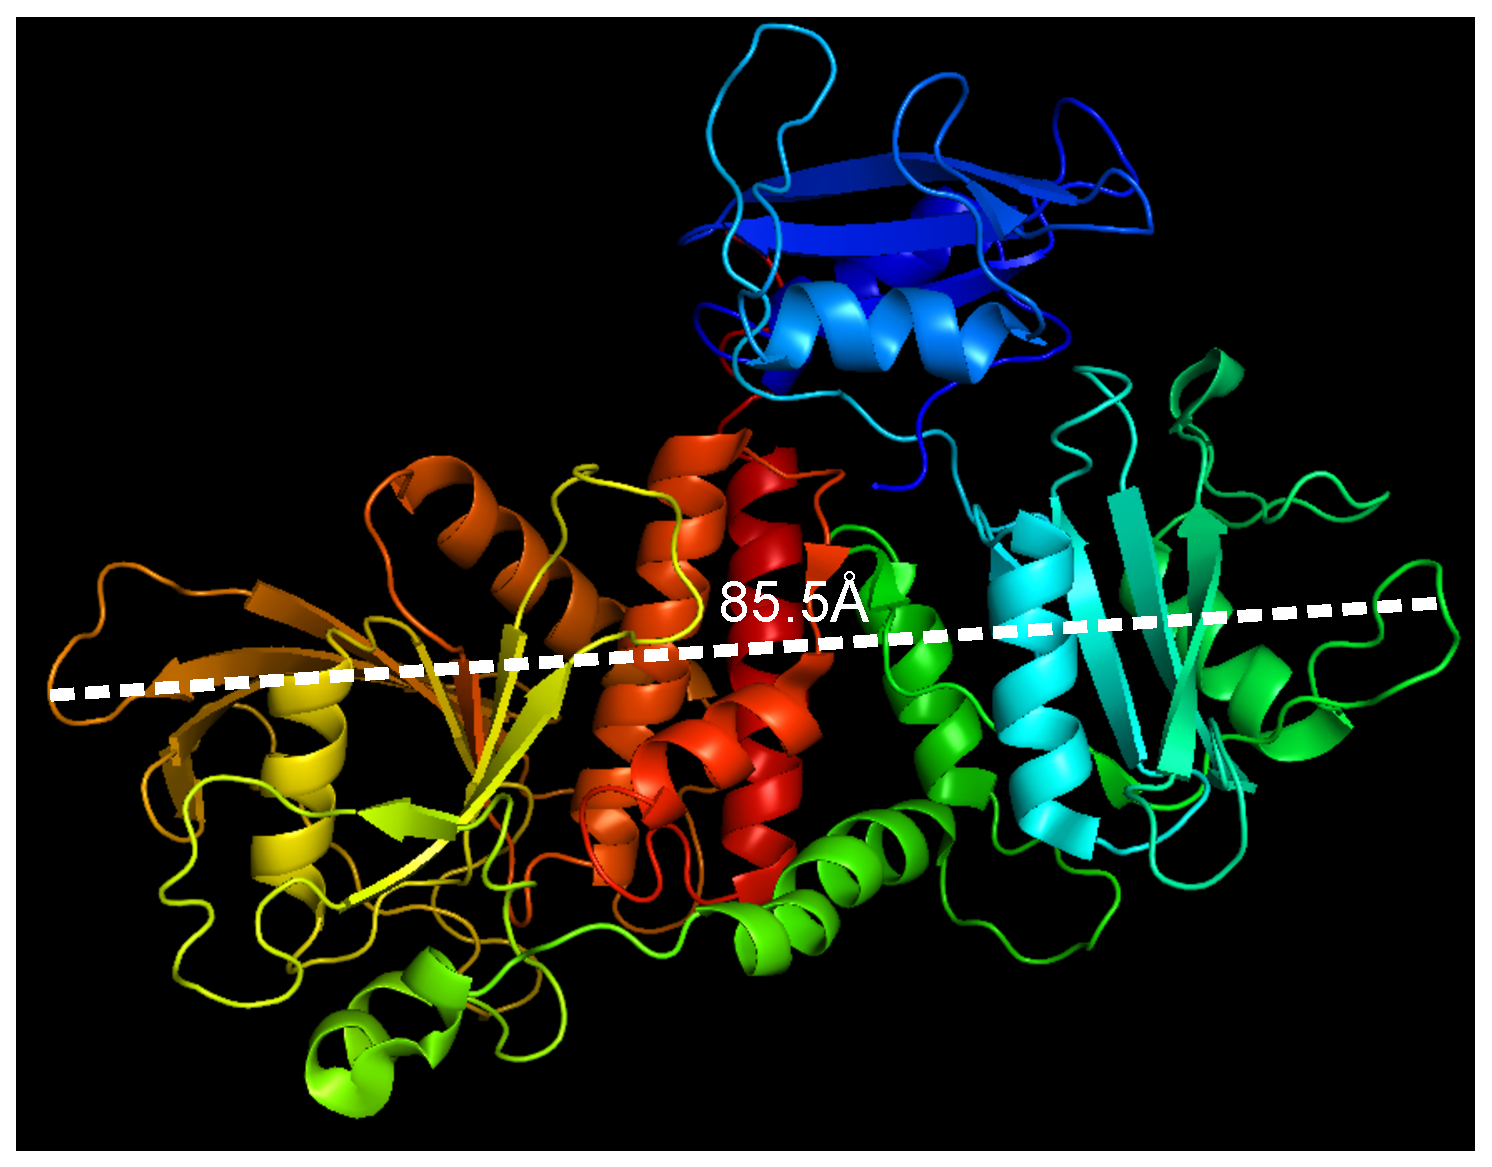
\includegraphics[width=0.5\linewidth]{ResultsFigures/SHP1PyMol/Diagonal1.eps}
\end{center}
\caption{Measurement of maximum length of SHP-1 (PDB 3PS5). \label{fig: SHP1Diag}}
\end{figure}

Alternatively, we can estimate the volume of SHP-1 as a rectangular prism and then create a spherical approximation of equal volume. We estimate the length, width and depth of SHP-1 to be 76\AA, 36\AA, and 58\text{\AA} respectively, giving a volume of 158688\AA$^3$. (Fig. \ref{fig: SHP1Rectangle}) From this, we calculate the radius for a spherical approximation to be 3.4nm.

\begin{figure}[H]
\begin{center}
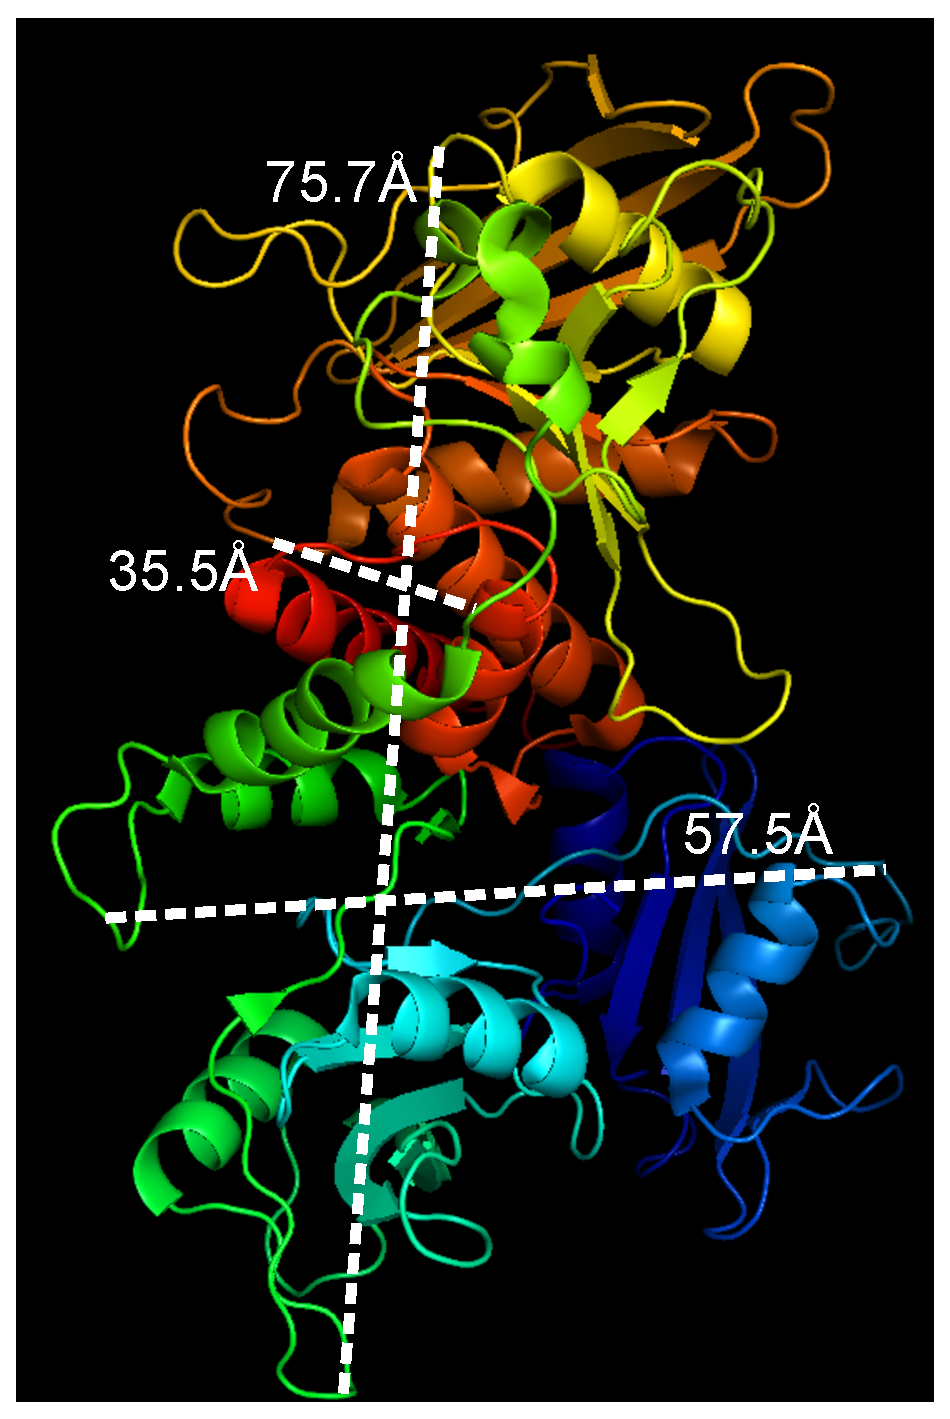
\includegraphics[width=0.4\linewidth]{ResultsFigures/SHP1PyMol/LengthWidthDepth.eps}
\end{center}
\caption{Measurement of rectangular dimensions of SHP-1 (PDB 3PS5). \label{fig: SHP1Rectangle} }
\end{figure}

% description of simulation - polymer-c code
Using the parameters estimated above, we simulate two equivalent tethers. The idealized SHP1 sphere, or ligand, is bound to the end of one of the tethers. The bound ligand is simulated as an idealized sphere which rotates with the tether. The bound ligand may not occupy the same space as the tether nor may it penetrate the surface if present. The second tether has a ghost ligand attached in the same location. (Fig. \ref{fig: LocalConcCartoon}) We allow each tether to explore conformation space, at each conformation determining if the ghost ligand is occluded by the rest of the tether, or in half-space, by the surface. For the tether with the ghost ligand, we record both the location of the center of the ligand and whether or not it was occluded at each conformation. For the tether with the bound ligand, we only record the location. For these simulations, we assume the two tethers are independent and do not sterically influence each other.

%% Diagram of simulation
\begin{figure}
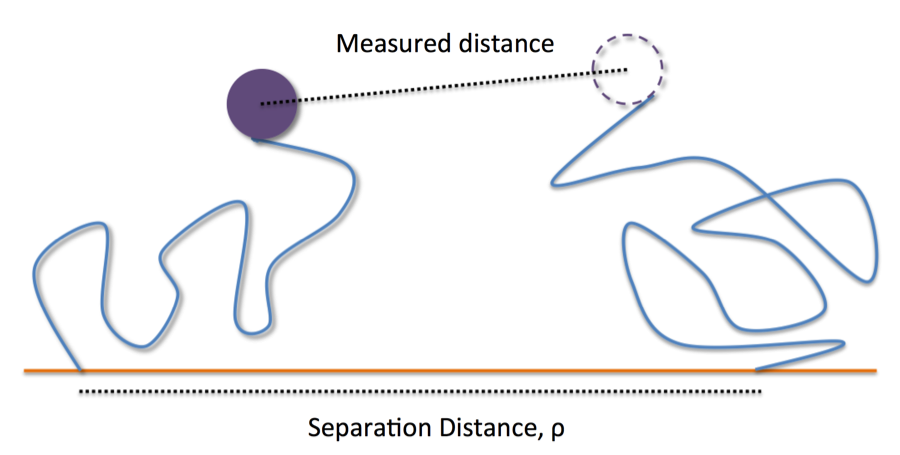
\includegraphics[width=\linewidth]{Diagram.png}
\caption{Cartoon of local concentration simulation in half space. \label{fig: LocalConcCartoon}}
\end{figure}

% description of simulation - matlab code
We compute the local concentration as the probability that the bound ligand is near the binding site (where near is defined by within some small radius) and the binding site is not occluded by the rest of the polymer. To calculate this, we separate the the tethers from each other by a distance, $\rho$, measured in Kuhn lengths by adding $\rho$ to the $x$-coordinate of the ghost ligand. We then measure the distance between the centers of the bound and ghost ligands. If the centers are within a cutoff distance from each other AND the ghost sphere is not occluded, then the bound ligand is able to bind. The local concentration is calculated by dividing the probability the ligand can bind by the volume of the sphere defined by the cutoff radius.


% description of curve fitting
% could cite Lagarias et al for Nelder-Mead algorithm?
We fit the local concentration curves to a half-gaussian curve, $\sigma_{fit}(\rho) = \sigma_{max}*e^{-\rho^2/l^2}$, as a function of the separation distance between the two tethers. To fit the simulated data, we use Matlab's fminsearch function which uses the Nelder-Mead simplex algorithm. The parameters found by the Nelder-Mead algorithm consistently give a smaller sum of least squares than parameters found using Trust-Region-Reflective Least Squares Algorithm or those found by heuristically sweeping parameter space to minimize the sum of least squares.


%
%The theoretical local concentration for two tethers a distance $\rho$ apart can be given by the following equation if both tethers are perfect worm-like chains:
%
%\begin{equation}
%    \sigma_{WLC}(\rho) = \left(\frac{3}{2\pi}\right)^{3/2} \frac{1}{L^3}e^{-\frac{3\rho^2}{2L^2}}
%\end{equation}
%
%Experimentally, we measure the reaction rate $R(\rho)$. This equation is the product of a $k_{cat}$ and $\sigma(\rho)$. If the two tethers were perfect worm-like chains and the attached ligand did not impact the local concentration then when we fit the experimental $R(\rho)$ to $\sigma_{WLC}(\rho)$, we would have $R(\rho) = k^{true}_{cat}*\sigma_{WLC}(\rho)$. However, since this is unlikely to be the case, if we fit to the WLC theory curve anyway, then we actually have $R(\rho) = k^{false}_{cat}*\sigma_{WLC}(\rho)$. Instead, if we consider our simulated data to be the true local concentration and we fit a half-gaussian curve, $\sigma_{fit}(\rho)$, to the data, then we would have $R(\rho) = k^{true}_{cat}*\sigma_{fit}(\rho)$, where $\sigma_{fit}(\rho) = a*e^{-\rho^2/c^2}$.
%
%We can use the simulated data to give an estimate of how incorrect $k^{false}_{cat}$ is compared to $k^{true}_{cat}$. We'll call this ratio $\kappa_{cat}$. Since we measured $R(\rho)$ experimentally, we must have:
%
%\todo{This doesn't look super pretty}
%
%\begin{align*}
%R(\rho) &= R(\rho) \\
%k^{false}_{cat}*\sigma_{WLC}(\rho, L) &= k^{true}_{cat}*\sigma_{fit}(\rho, a, c) \\
%\kappa_{cat} = \frac{k^{false}_{cat}}{k^{true}_{cat}} &= \frac{\sigma_{fit}(\rho, a, c)}{\sigma_{WLC}(\rho, L)} \\
%\kappa_{cat} &= \frac{a*e^{-\rho^2/c^2}}{\left(\frac{3}{2\pi}\right)^{3/2} \frac{1}{L^3}e^{-\frac{3\rho^2}{2L^2}}} \\
%\kappa_{cat} &= \frac{aL^3}{\left(\frac{3}{2\pi}\right)^{3/2}} \\
%\kappa_{cat} &= \frac{a\left(\sqrt{\frac{3}{2}}c\right)^3}{\left(\frac{3}{2\pi}\right)^{3/2} } \\
%\kappa_{cat} &= ac^3\pi^{3/2}\\
%\end{align*}
%
%if we \hl{assume? note?} $c^2 = \sqrt{\frac{2}{3}}L^2 \implies L = \sqrt{\frac{3}{2}}c$.
%
%%summary table of possible fits to experimental data
%\begin{center}
%\begin{tabular}{| c | c | c |}
%    \hline
%        Model & Truth & Result \\ 
%        \hline 
%        Worm-like chain     &   T   &   $R(\rho) = k^{true}_{cat}*\sigma_{WLC}(\rho)$    \\
%        & & \\
%        Worm-like chain     &   F   &   $R(\rho) = k^{false}_{cat}*\sigma_{WLC}(\rho)$   \\ 
%        & & \\
%        Half-gaussian fit   &   T   &   $R(\rho) = k^{true}_{cat}*\sigma_{fit}(\rho)$    \\
%    \hline
%\end{tabular}
%\end{center}
%
%
%We must therefore find appropriate $\sigma_{max}$ and $l$ values for our half-gaussian fit in order to calculate the error.



%%%%%%%%%%%%%%%%%%%%%%%%%%%%%%%%%%%%%%%%%%%%%%%%%%%%%%%%%%%%%%%%%%%%%%%%%%%%%%%%%%%%%%%%%%%%%%%%%%%%%
%%%%%%%%%%%%%%%%%%%%%%%%%%%%%%%%%%%%%%%%%%%%%%%%%%%%%%%%%%%%%%%%%%%%%%%%%%%%%%%%%%%%%%%%%%%%%%%%%%%%%
\subsection{Results}

\subsubsection{Accessibility of a reaction site is reduced by the presence of a surface}

We first investigate the accessibility of a binding site at the end of the polymer when a surface is present. We record how often the membrane causes the binding site to be inaccessible to its ligand, as opposed to occlusion by the rest of the polymer. We find that occlusion caused only by the membrane increases with the size of the ligand, but decreases with longer polymers (Fig. \ref{fig: MembraneOcclusionVSNVSR}). 

We next investigate how the presence of a surface impacts binding of a ligand to a single tether compared to in free-space. We find that a surface consistently net decreases the probability a ligand can bind to a tether, irrespective of tether length or ligand size. For long tethers, the surface reduction is minimal, in some parameters almost eliminating the difference. A larger ligand creates a larger fold decrease in the ability of the kinase to bind in half-space. (Fig. \ref{fig: OcclusionVSN})

\begin{figure}[h]
       \begin{center}
       		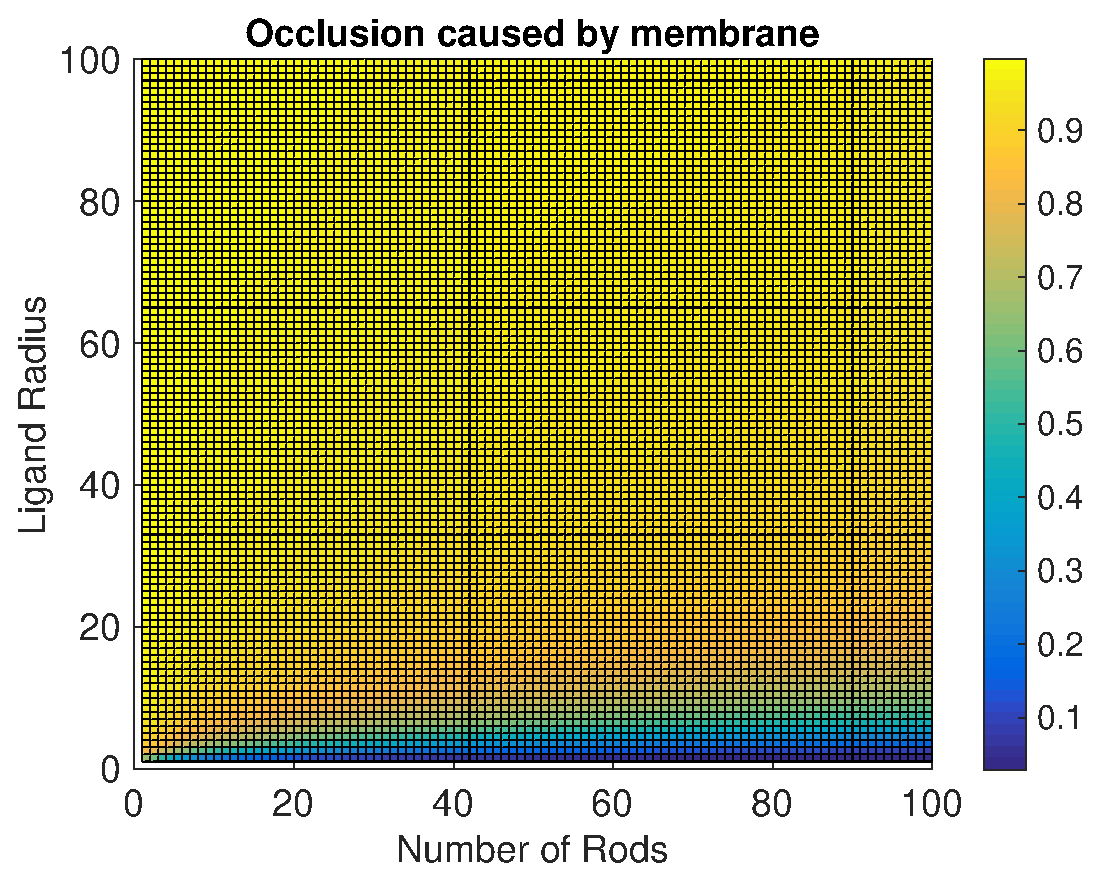
\includegraphics[width=0.7\linewidth]{ResultsFigures/MembraneCausedOcclusion/MembraneCausedOcclusionVSNVSirLigand.eps}
       \end{center}
       \caption{Probability of binding site occlusion due to presence of a surface as a function of polymer length and ligand radius. \label{fig: MembraneOcclusionVSNVSR}}
\end{figure}

\begin{figure}[h]
    \begin{center}
        \begin{subfigure}{\linewidth}
        		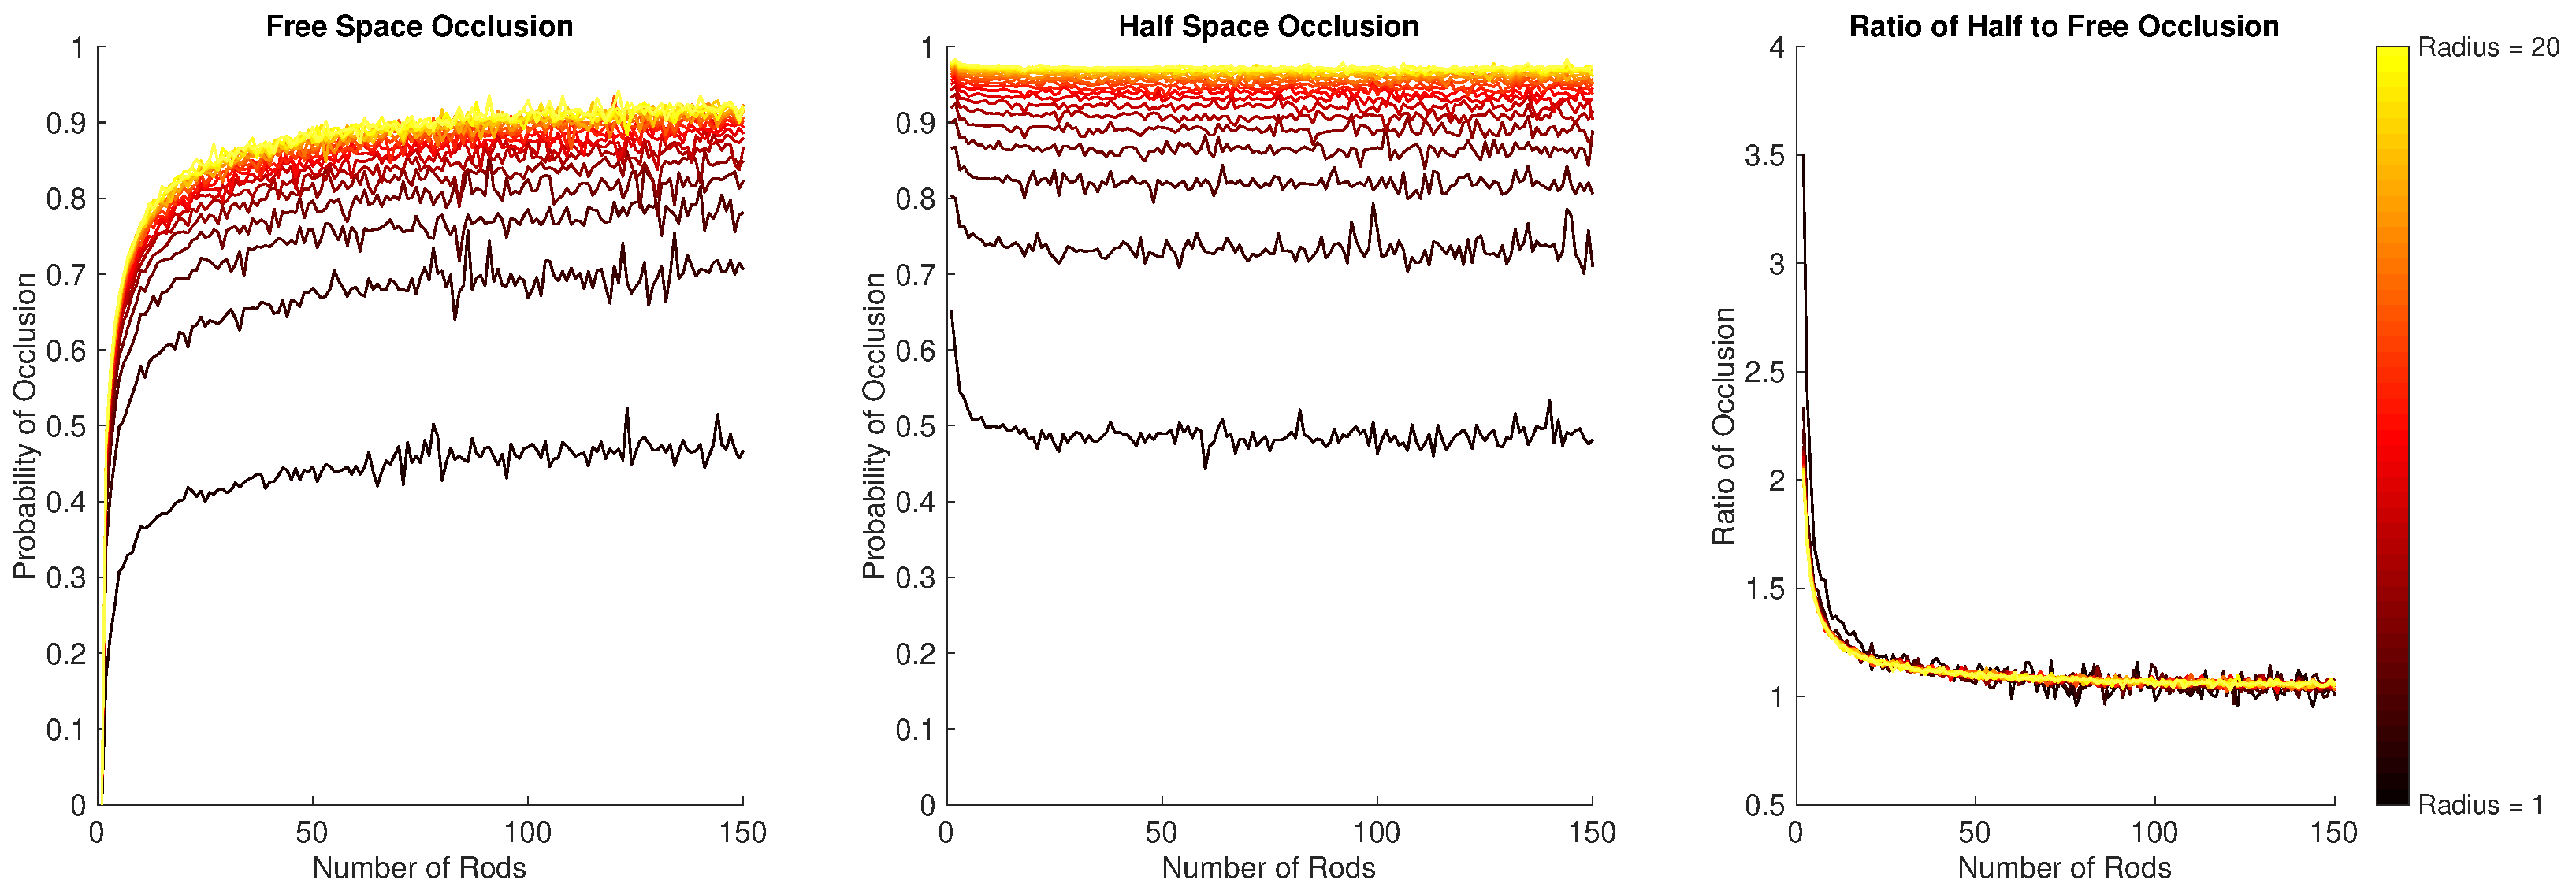
\includegraphics[width=\linewidth]{ResultsFigures/BindingSurfaceFactor/OcclusionVSN.eps}
        		\caption{}
        \end{subfigure}
        	\begin{subfigure}{\linewidth}
        		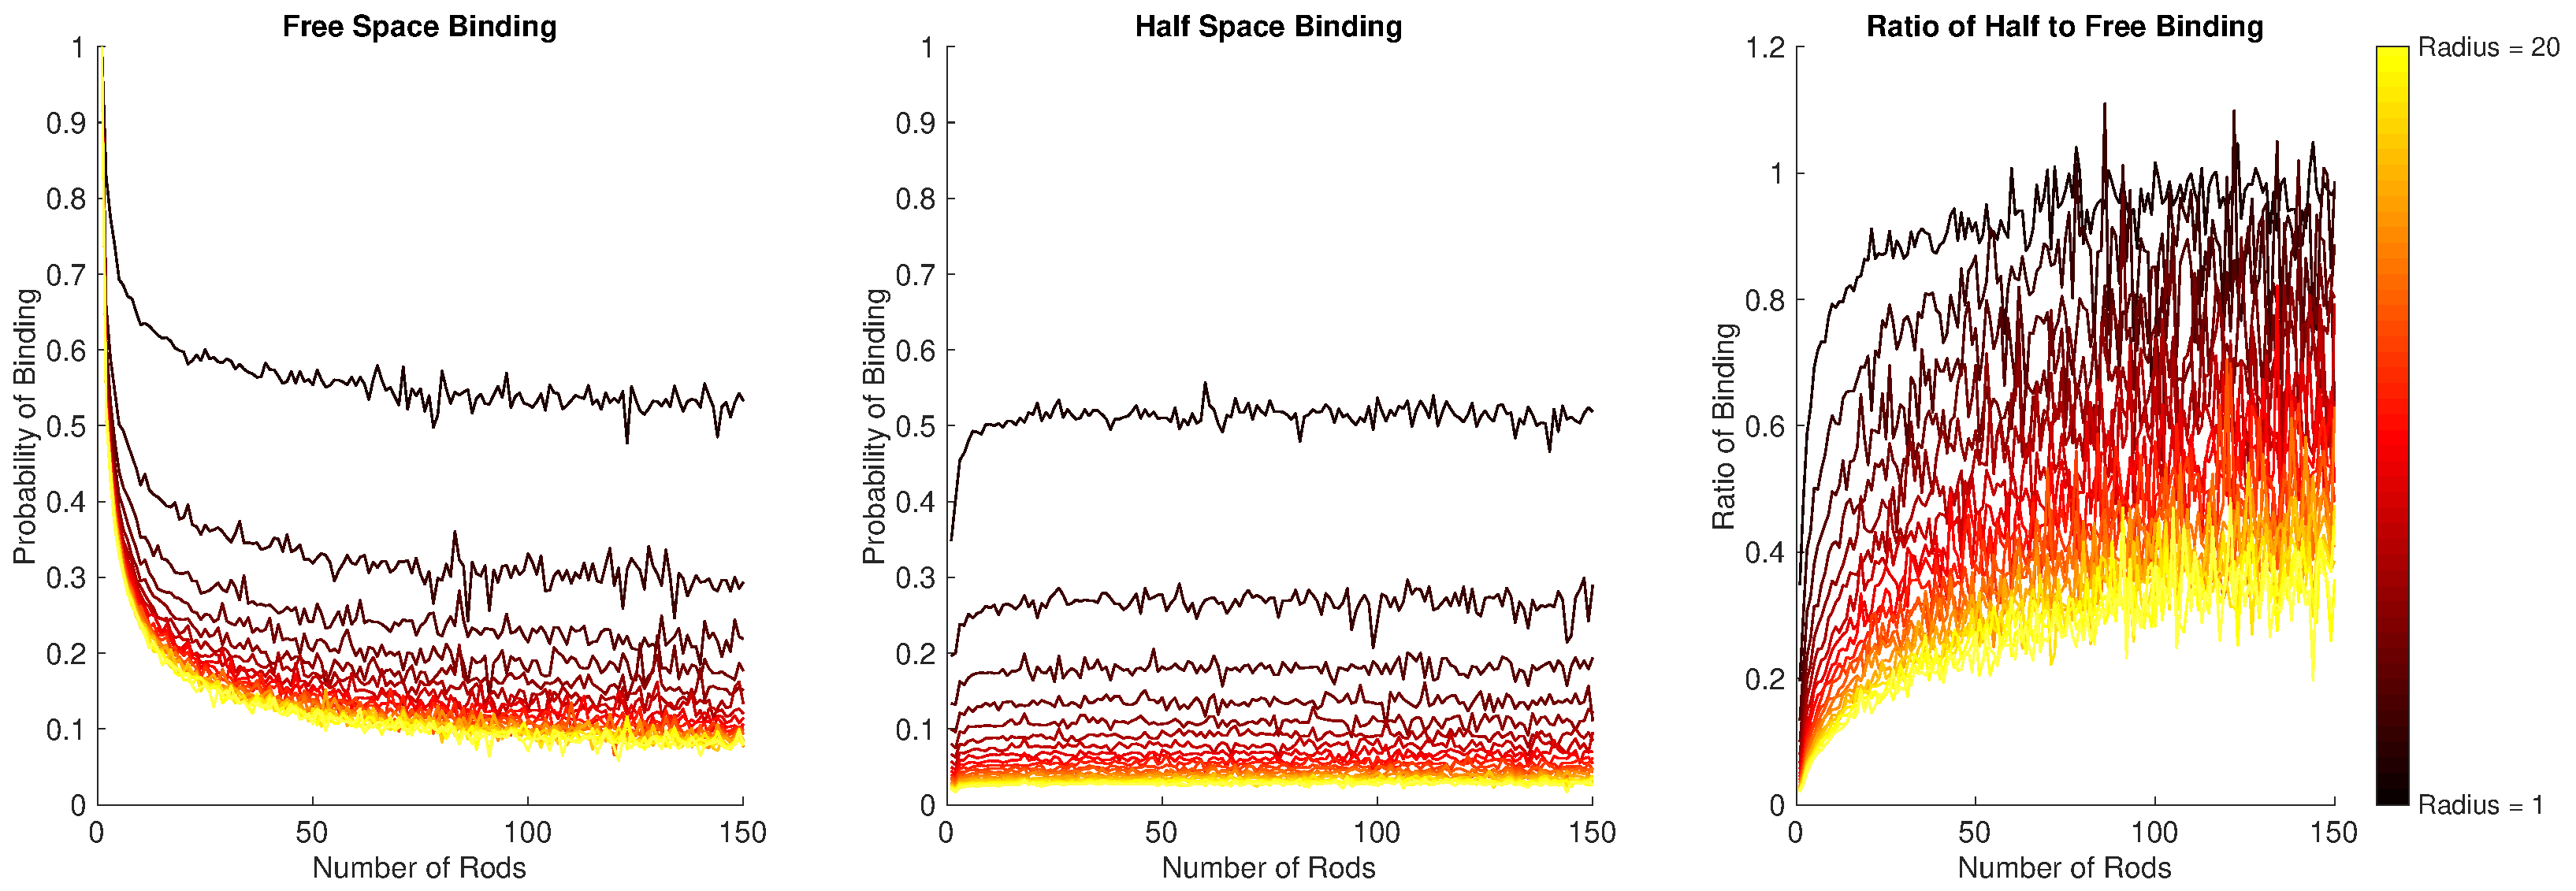
\includegraphics[width=\linewidth]{ResultsFigures/BindingSurfaceFactor/BindingVSN.eps}
        		\caption{}
        \end{subfigure}
        \caption{Probability of ligand being occluded, $p_{occ}$ (top row), and probability of ligand binding, $1-p_{occ}$ (bottom row), as a function of tether length for various ligand radii. Free-space (left column), half-space (middle), and the ratio of probabilities half-space to free-space (right). \label{fig: OcclusionVSN} }
       \end{center}
\end{figure}
       

\subsubsection{Future Work: Impact of membrane on reactions between tethered reactants}

% introduce effective concentration compared to standard concentration
For a reactant in solution, the reaction rate will be proportional to the concentration of the reactant. On the other hand, for a reaction between two tethered molecules, the reaction rate is proportional to the effective concentration \cite{VanValen2009,Bryant2017} (Cite - Vavylonis paper).
Effective concentration is defined as how often a ligand bound to the tail of one anchored polymer encounters a binding site on the tail of a second anchored polymer, taking into account the accessibility of the binding site. 
% future work
We will explore how effective concentration is impacted by ligand size and polymer length. We will generate plots of the effective concentration as function of separation distance in both free-space and half-space for multiple sizes of polymer and bound ligand. We expect these to look similar to the schematic shown in Fig. \ref{fig: ConcVSSeparation}. Under simplified circumstances, e.g. no bound ligand, it has been shown that the effective concentration will be a half-gaussian \cite{Goyette2017}. Therefore, we expect our plots to also resemble a half-gaussian. We will fit a half-gaussian to these curves and consider the change in maximum effective concentration and width of the curve (reach parameter) between free-space and half-space. 

% expectations of reach parameter
We have shown that a polymer in half-space will have a mildly extended end-to-end distribution compared to a polymer in free-space (Fig. \ref{fig: ReeHalfVSFree}). For this reason, we expect only a mild change in the reach parameter between free-space and half-space. 

% expectations for maximum concentration
It is less clear what effect a surface will have on maximum concentration. 
	% - membrane should enhance by reducing space
	On the one hand, a membrane will force both polymers to occupy the same half space, which should enhance the effective concentration.
	% - membrane reducing ability to bind to site
	On the other hand, we have seen that presence of a membrane reduces the accessibility of a binding site, decreasing effective concentration. 
	% - prediction
	We expect that for a small enough ligand, the membrane will lead to a net enhancement. We will answer whether, for a ligand of typical size, the membrane creates a net enhancement or reduction of the effective concentration.


%When ligand size is zero, or equivalent to no ligand attached to the polymer, then we see the free space polymers experience an effective concentration predicted by the worm-like chain model. Note that variability from the theoretical WLC curve is mitigated by decreasing the volume considered a binding encounter. We see that the surface enhances the effective concentration over the free space values when no ligand is present. When a large ligand is bound to one of the tethers, the presence of a membrane reduces the maximum effective concentration compared to in free-space. (Fig. \ref{fig: ConcVSSeparation}, Fig. \ref{fig: MaxEffConc}, Fig. \ref{MaxEffConcRatio})


\begin{figure}[h]
    \begin{center}
        		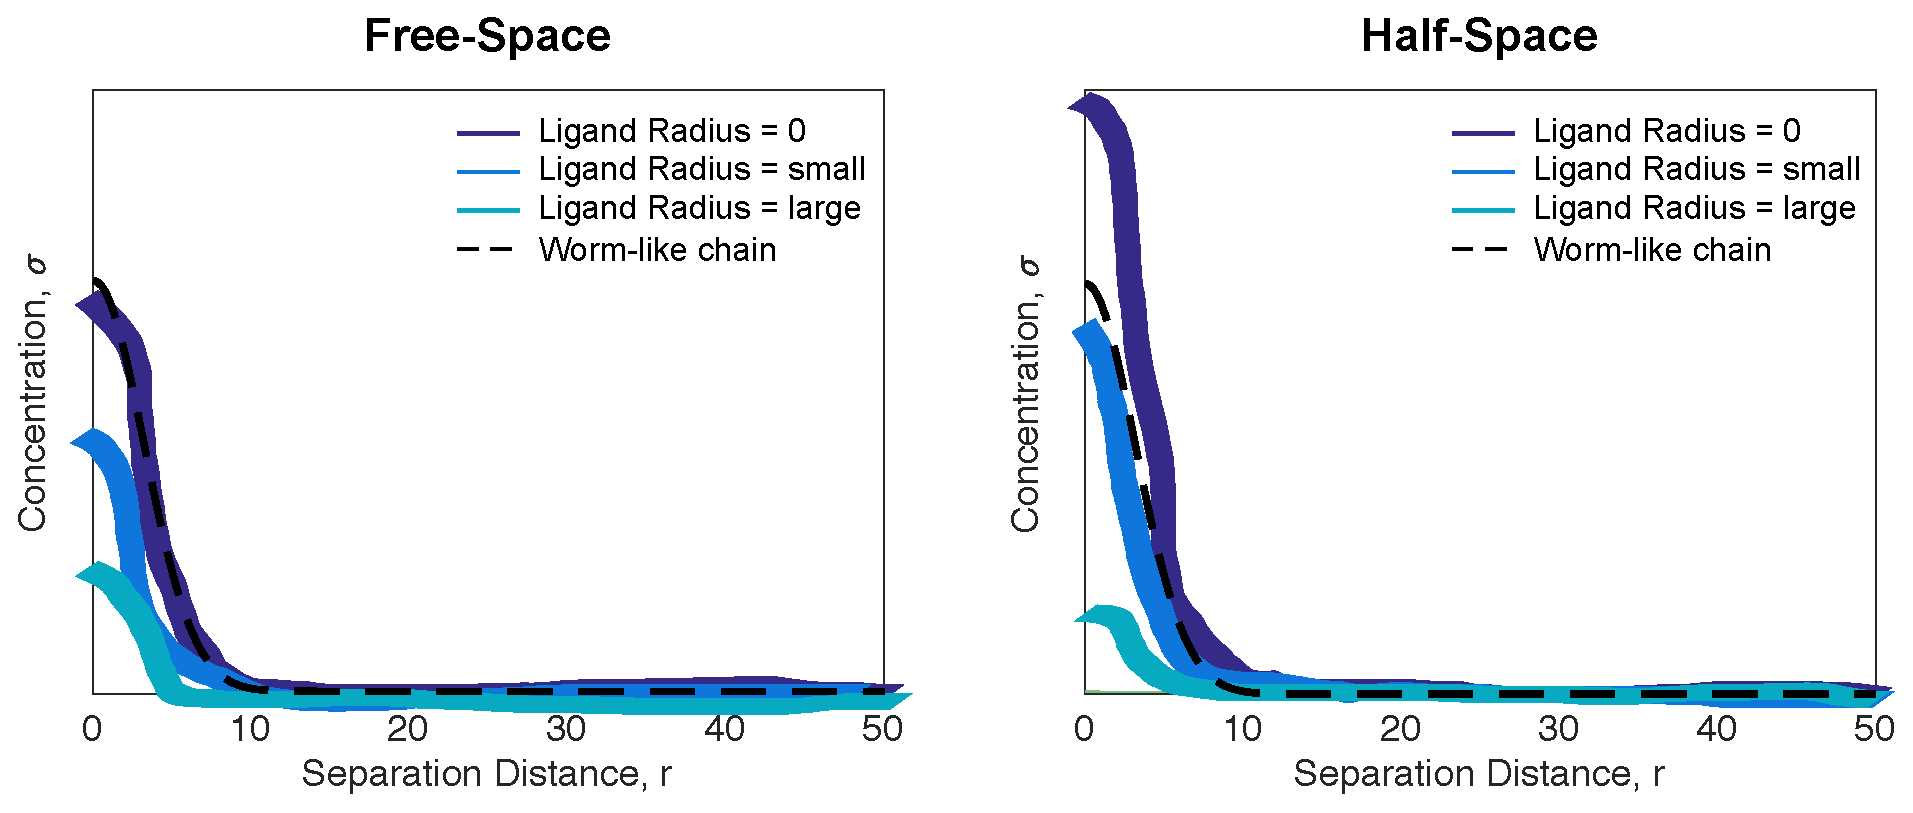
\includegraphics[width=0.85\linewidth]{ResultsFigures/EffectiveConcentrationKernel/ConcentrationVSSeparationCartoon.eps}
    \end{center}
    \caption{Possible plot of effective concentration as a function of tether separation distance. \label{fig: ConcVSSeparation}}
\end{figure}

%\begin{figure}[h]
%    \begin{center}
%        		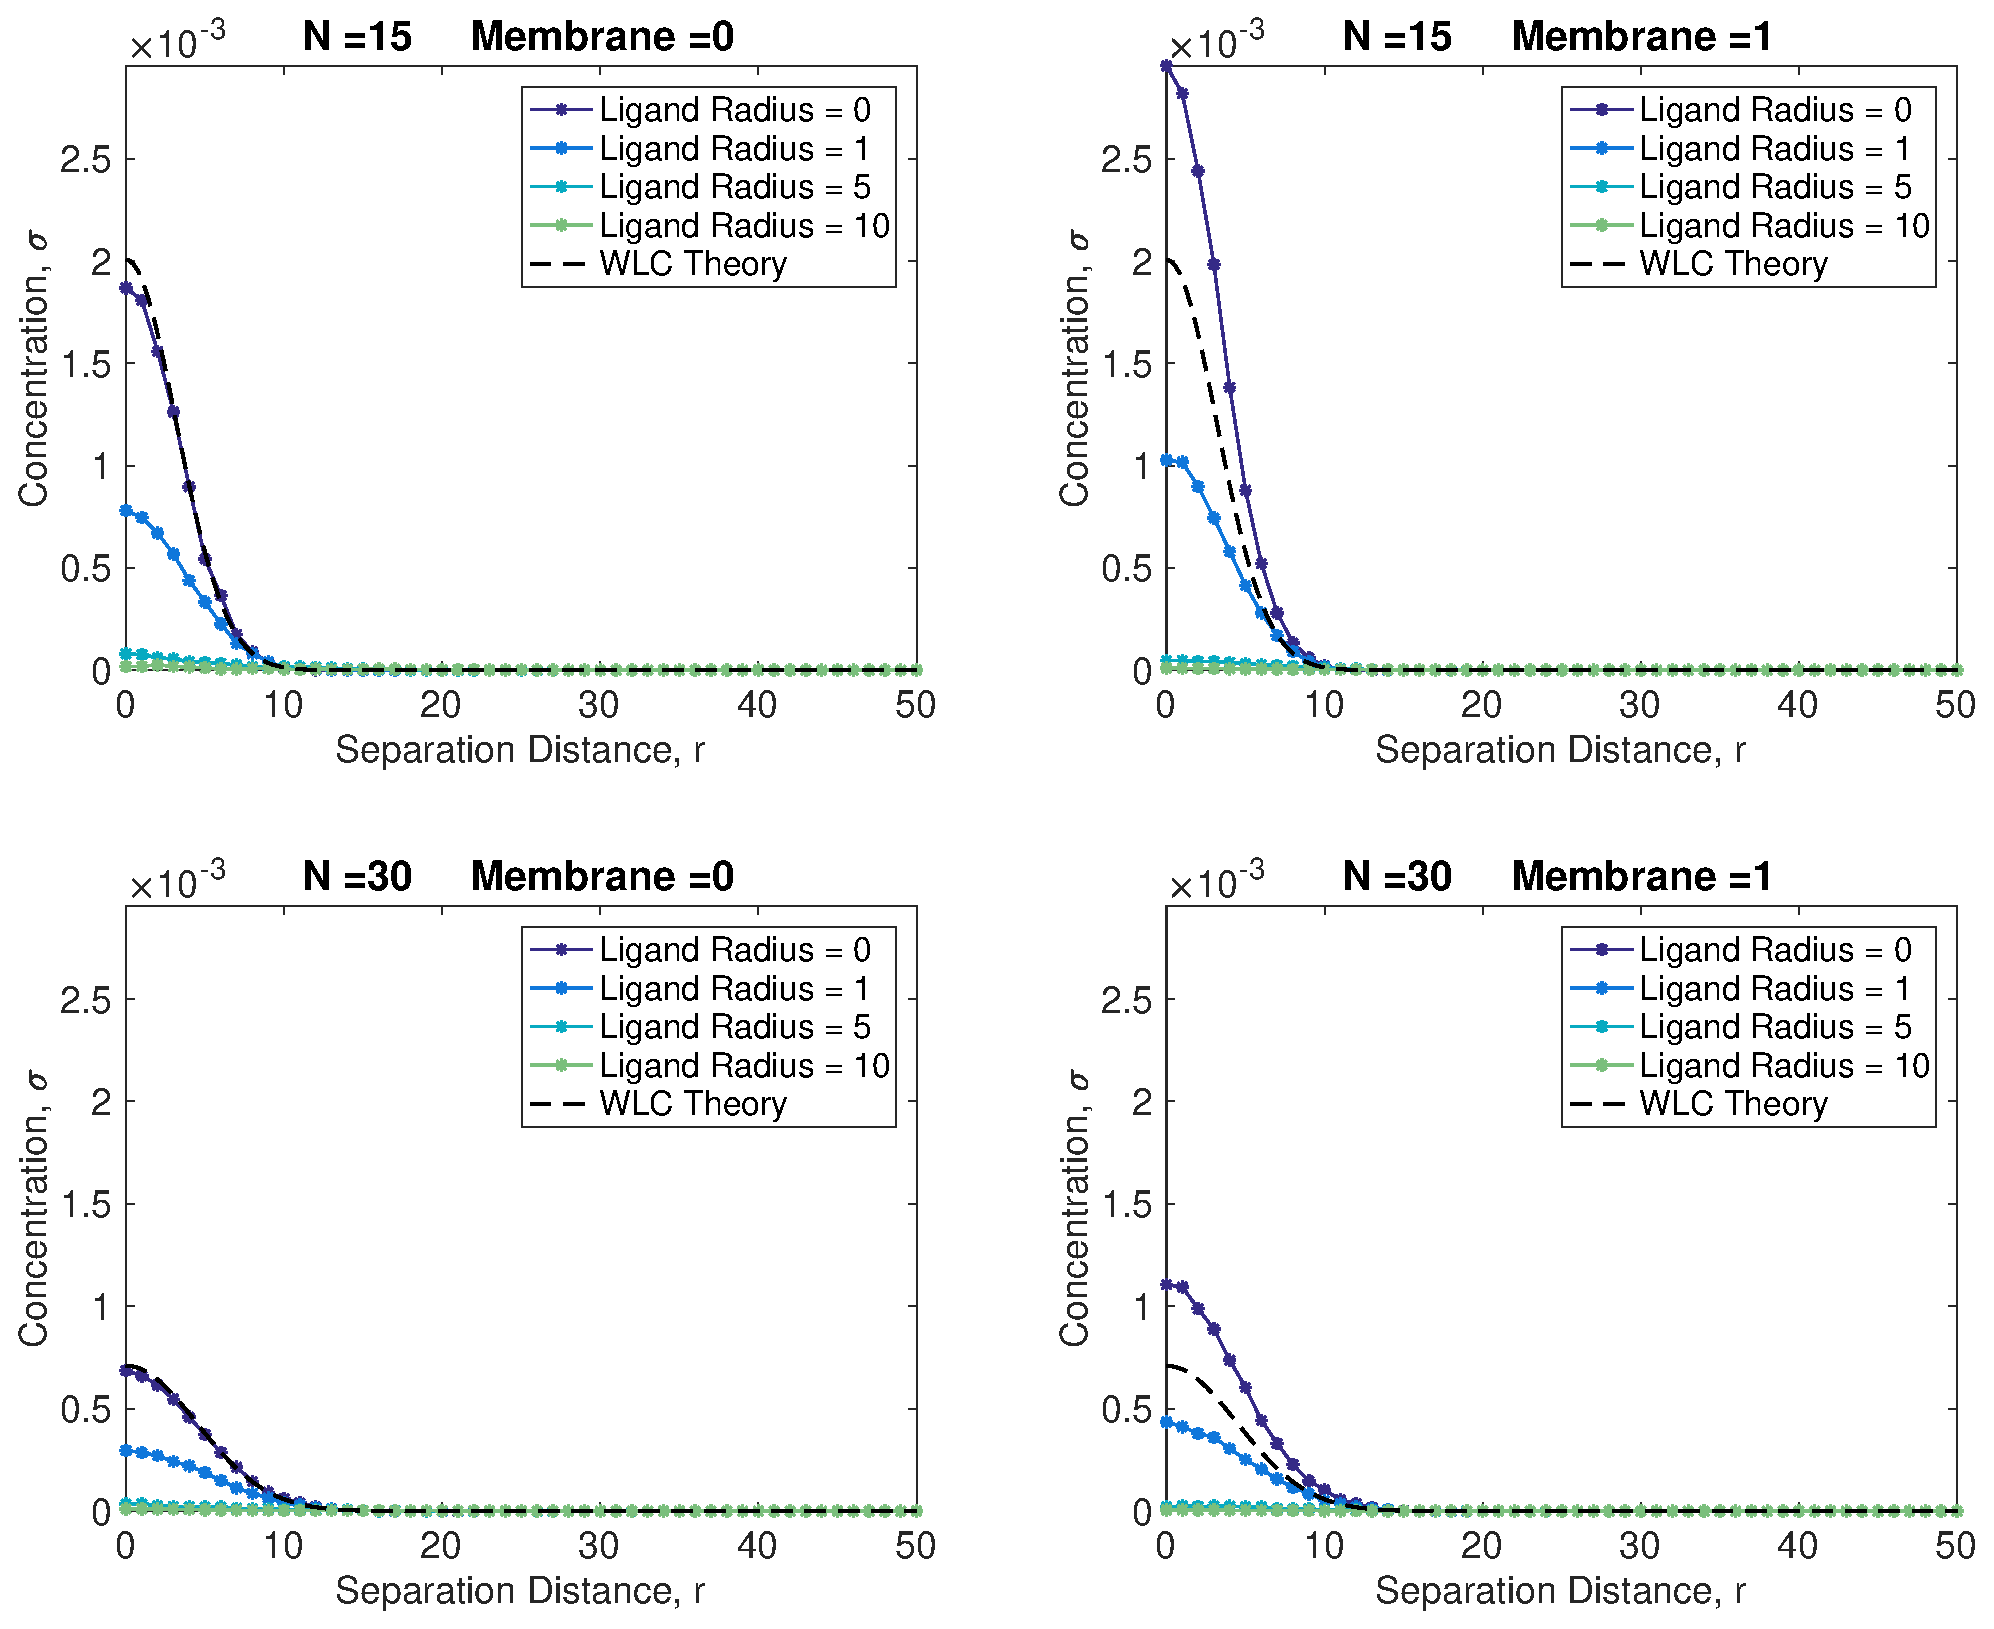
\includegraphics[width=0.7\linewidth]{ResultsFigures/EffectiveConcentrationKernel/ConcentrationVSSeparation.eps}
%        \caption{Effective concentration as a function of tether separation distance. \label{fig: ConcVSSeparation}}
%    \end{center}
%\end{figure}

%\begin{figure}[H]
%    \begin{center}
%        		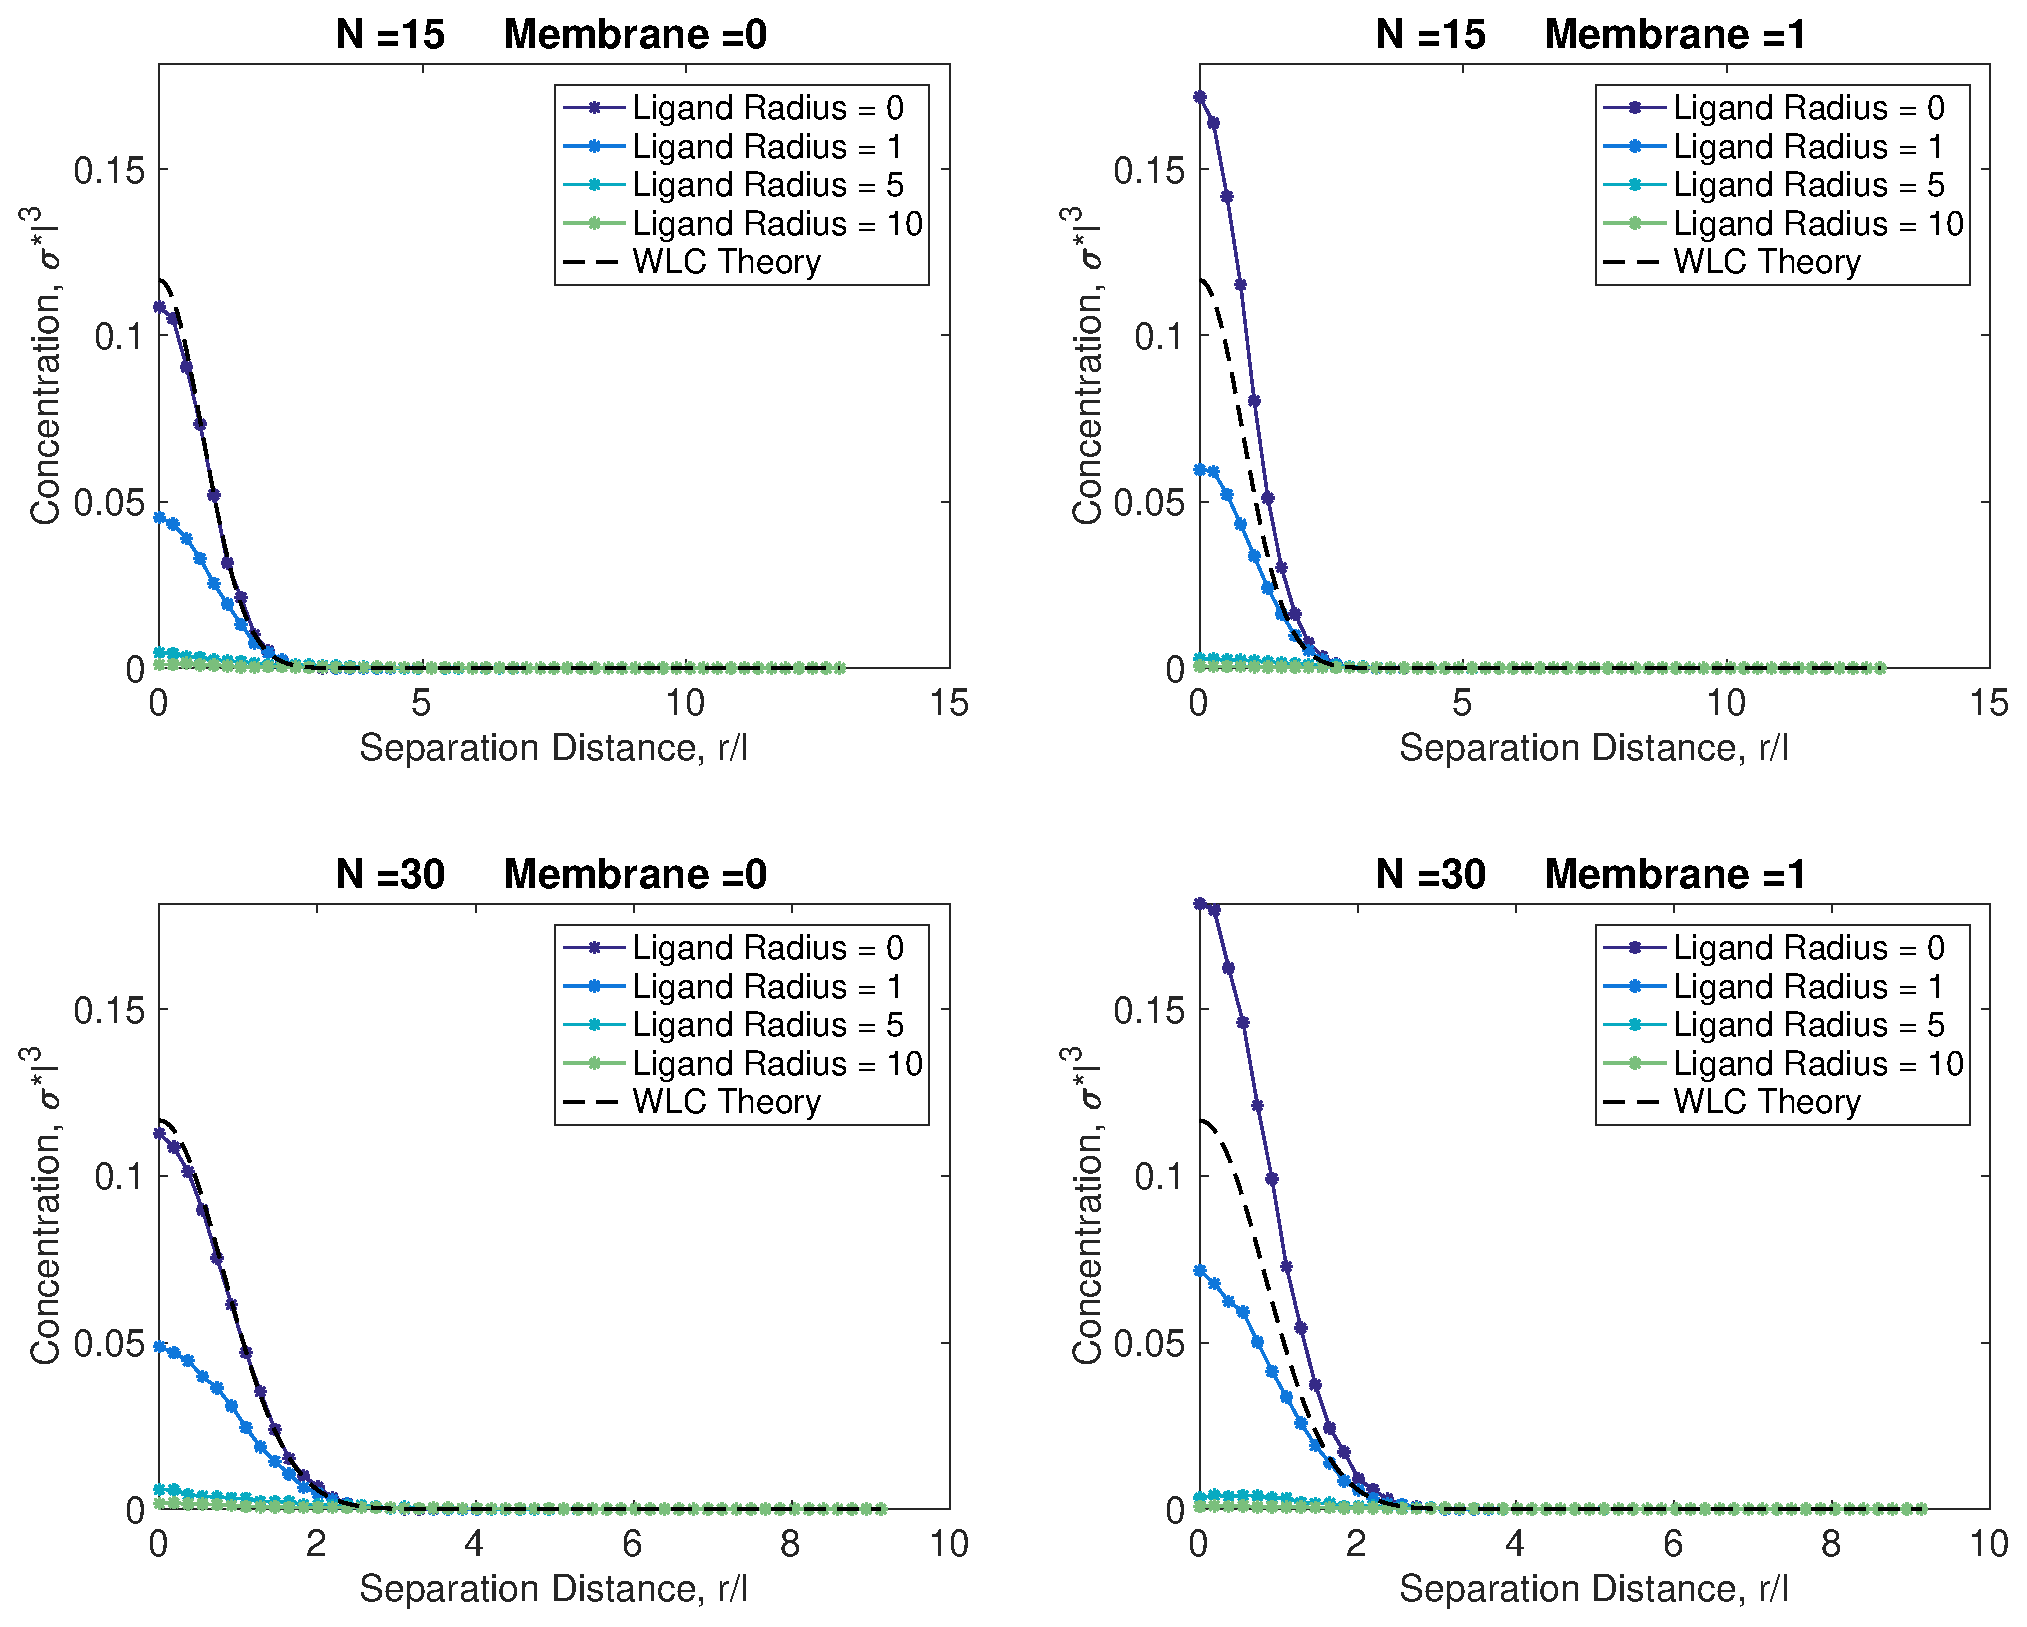
\includegraphics[width=0.8\linewidth]{ResultsFigures/EffectiveConcentrationKernel/ConcentrationNondimVSSeparation.eps}
%        \caption{}
%    \end{center}
%\end{figure}


%
%\begin{figure}[H]
%    \begin{center}
%        		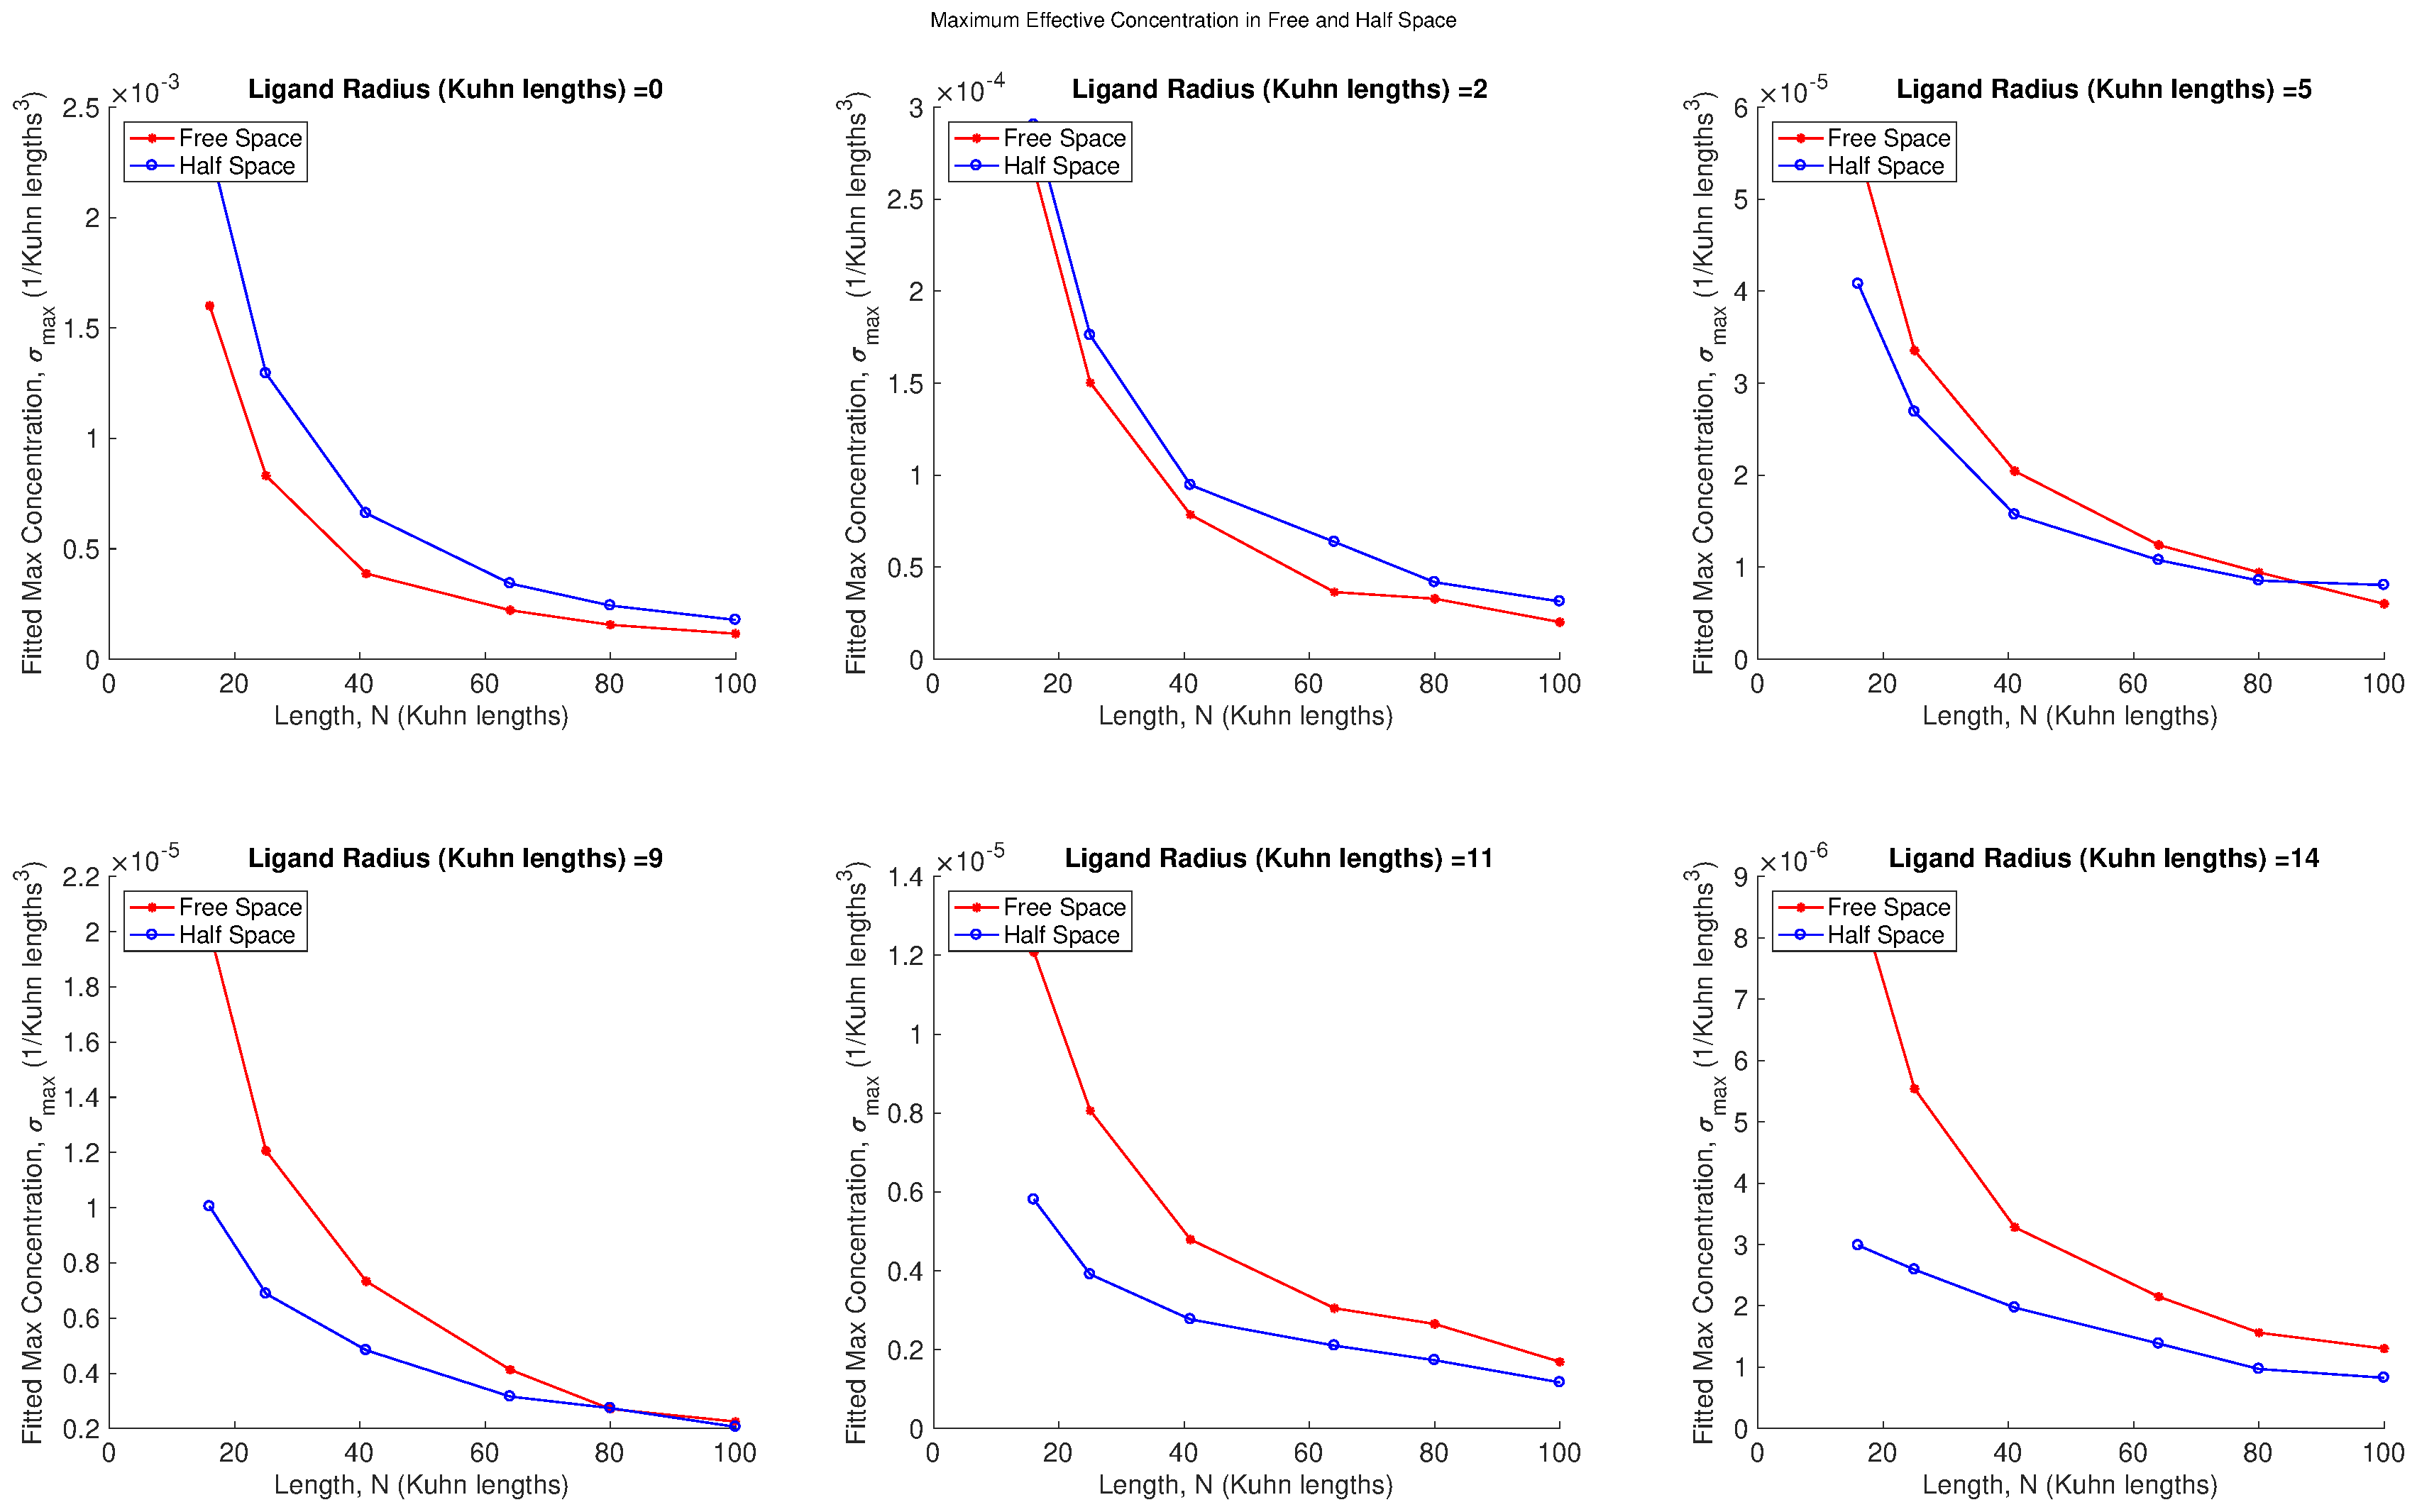
\includegraphics[width=\linewidth]{ResultsFigures/MaxEffConc/MaximumEffConcFreeHalf.eps}
%        \caption{Maximum effective concentration of half-gaussian fit to local concentration data plotted as a function of tether length, $N$ for various ligand radii in free-space (red) and half-space (blue). \label{fig: MaxEffConc}}
%    \end{center}
%\end{figure}
%
%\begin{figure}[H]
%    \begin{center}
%        		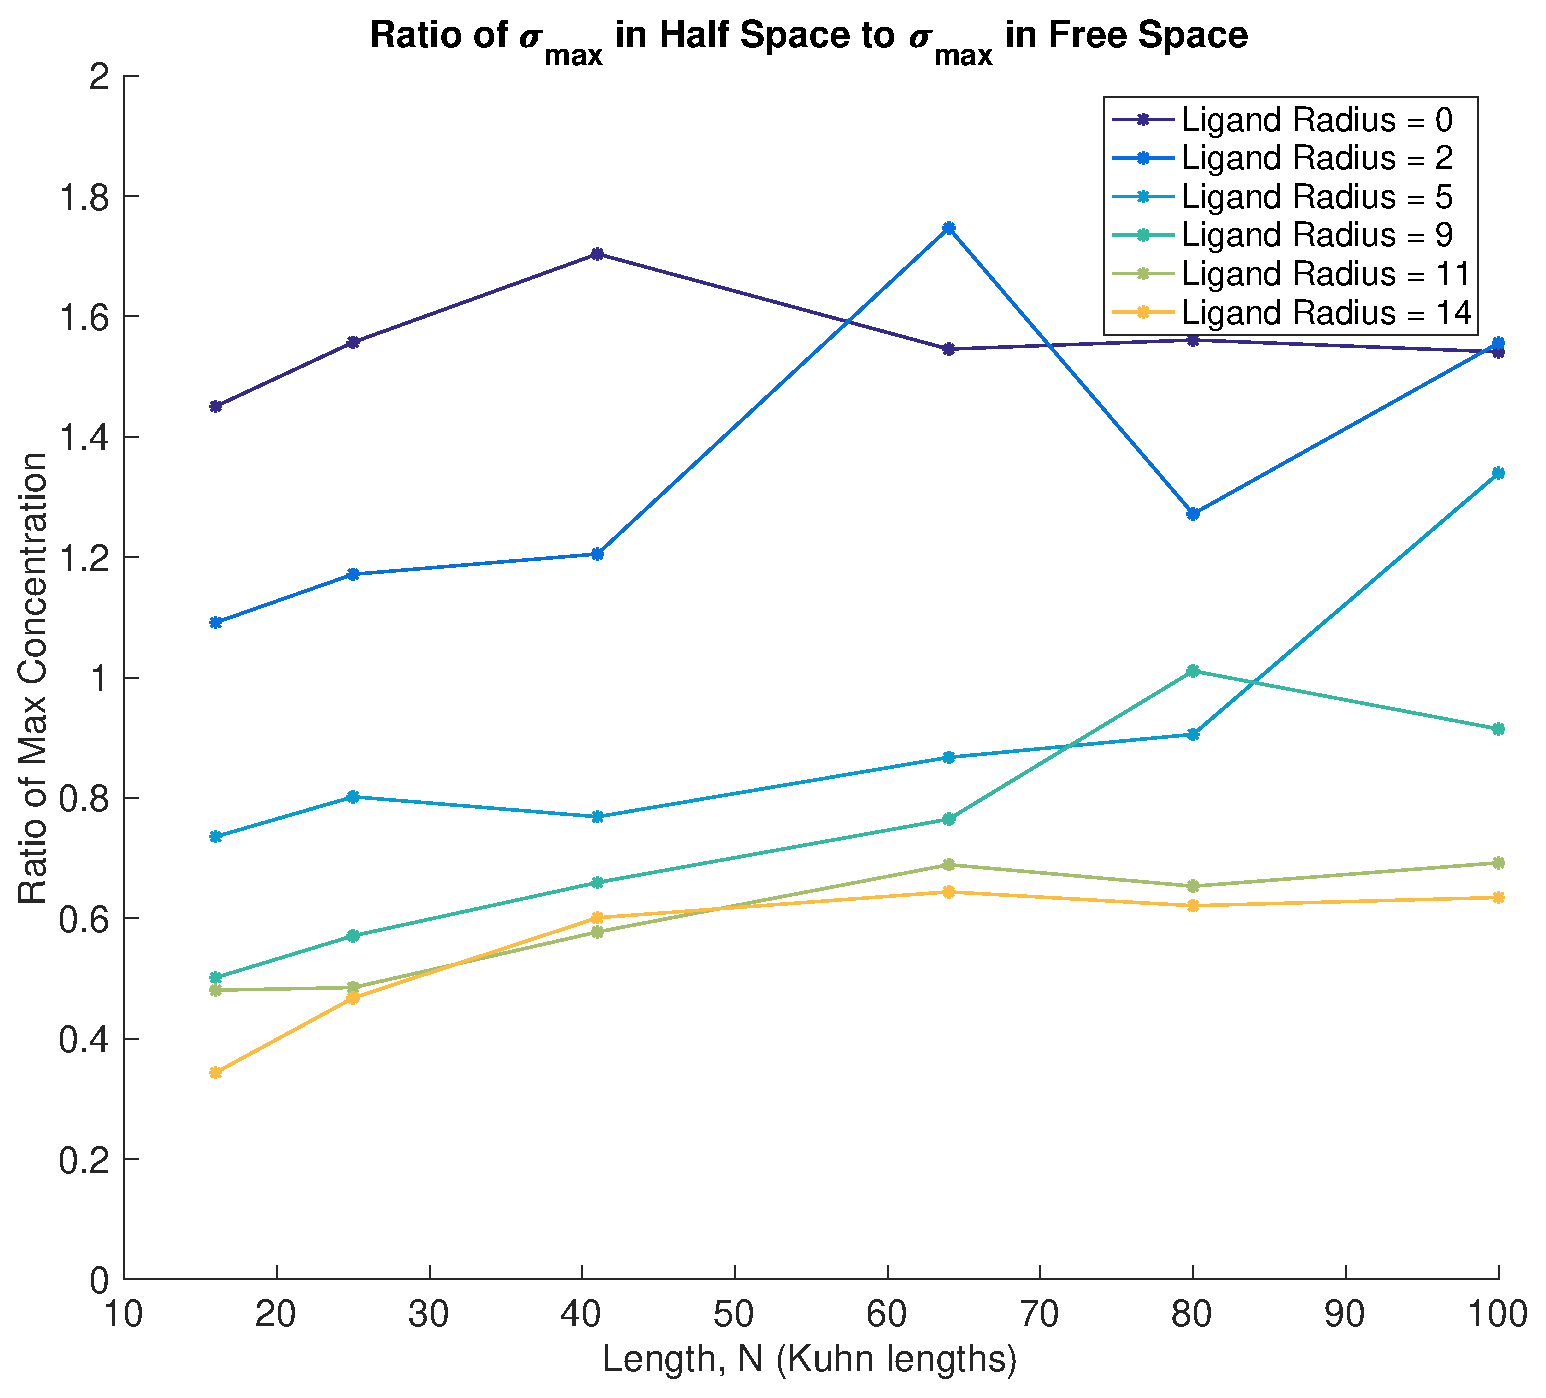
\includegraphics[width=0.7\linewidth]{ResultsFigures/MaxEffConc/MaximumEffConcRatio.eps}
%        \caption{Ratio of half-space fitted maximum effective concentration to free-space fitted maximum effective concentration as a function of tether length, $N$ (Kuhn lengths), for various ligand radii. \label{fig: MaxEffConcRatio}}
%    \end{center}
%\end{figure}


%\begin{figure}[H]
%    \begin{center}
%        		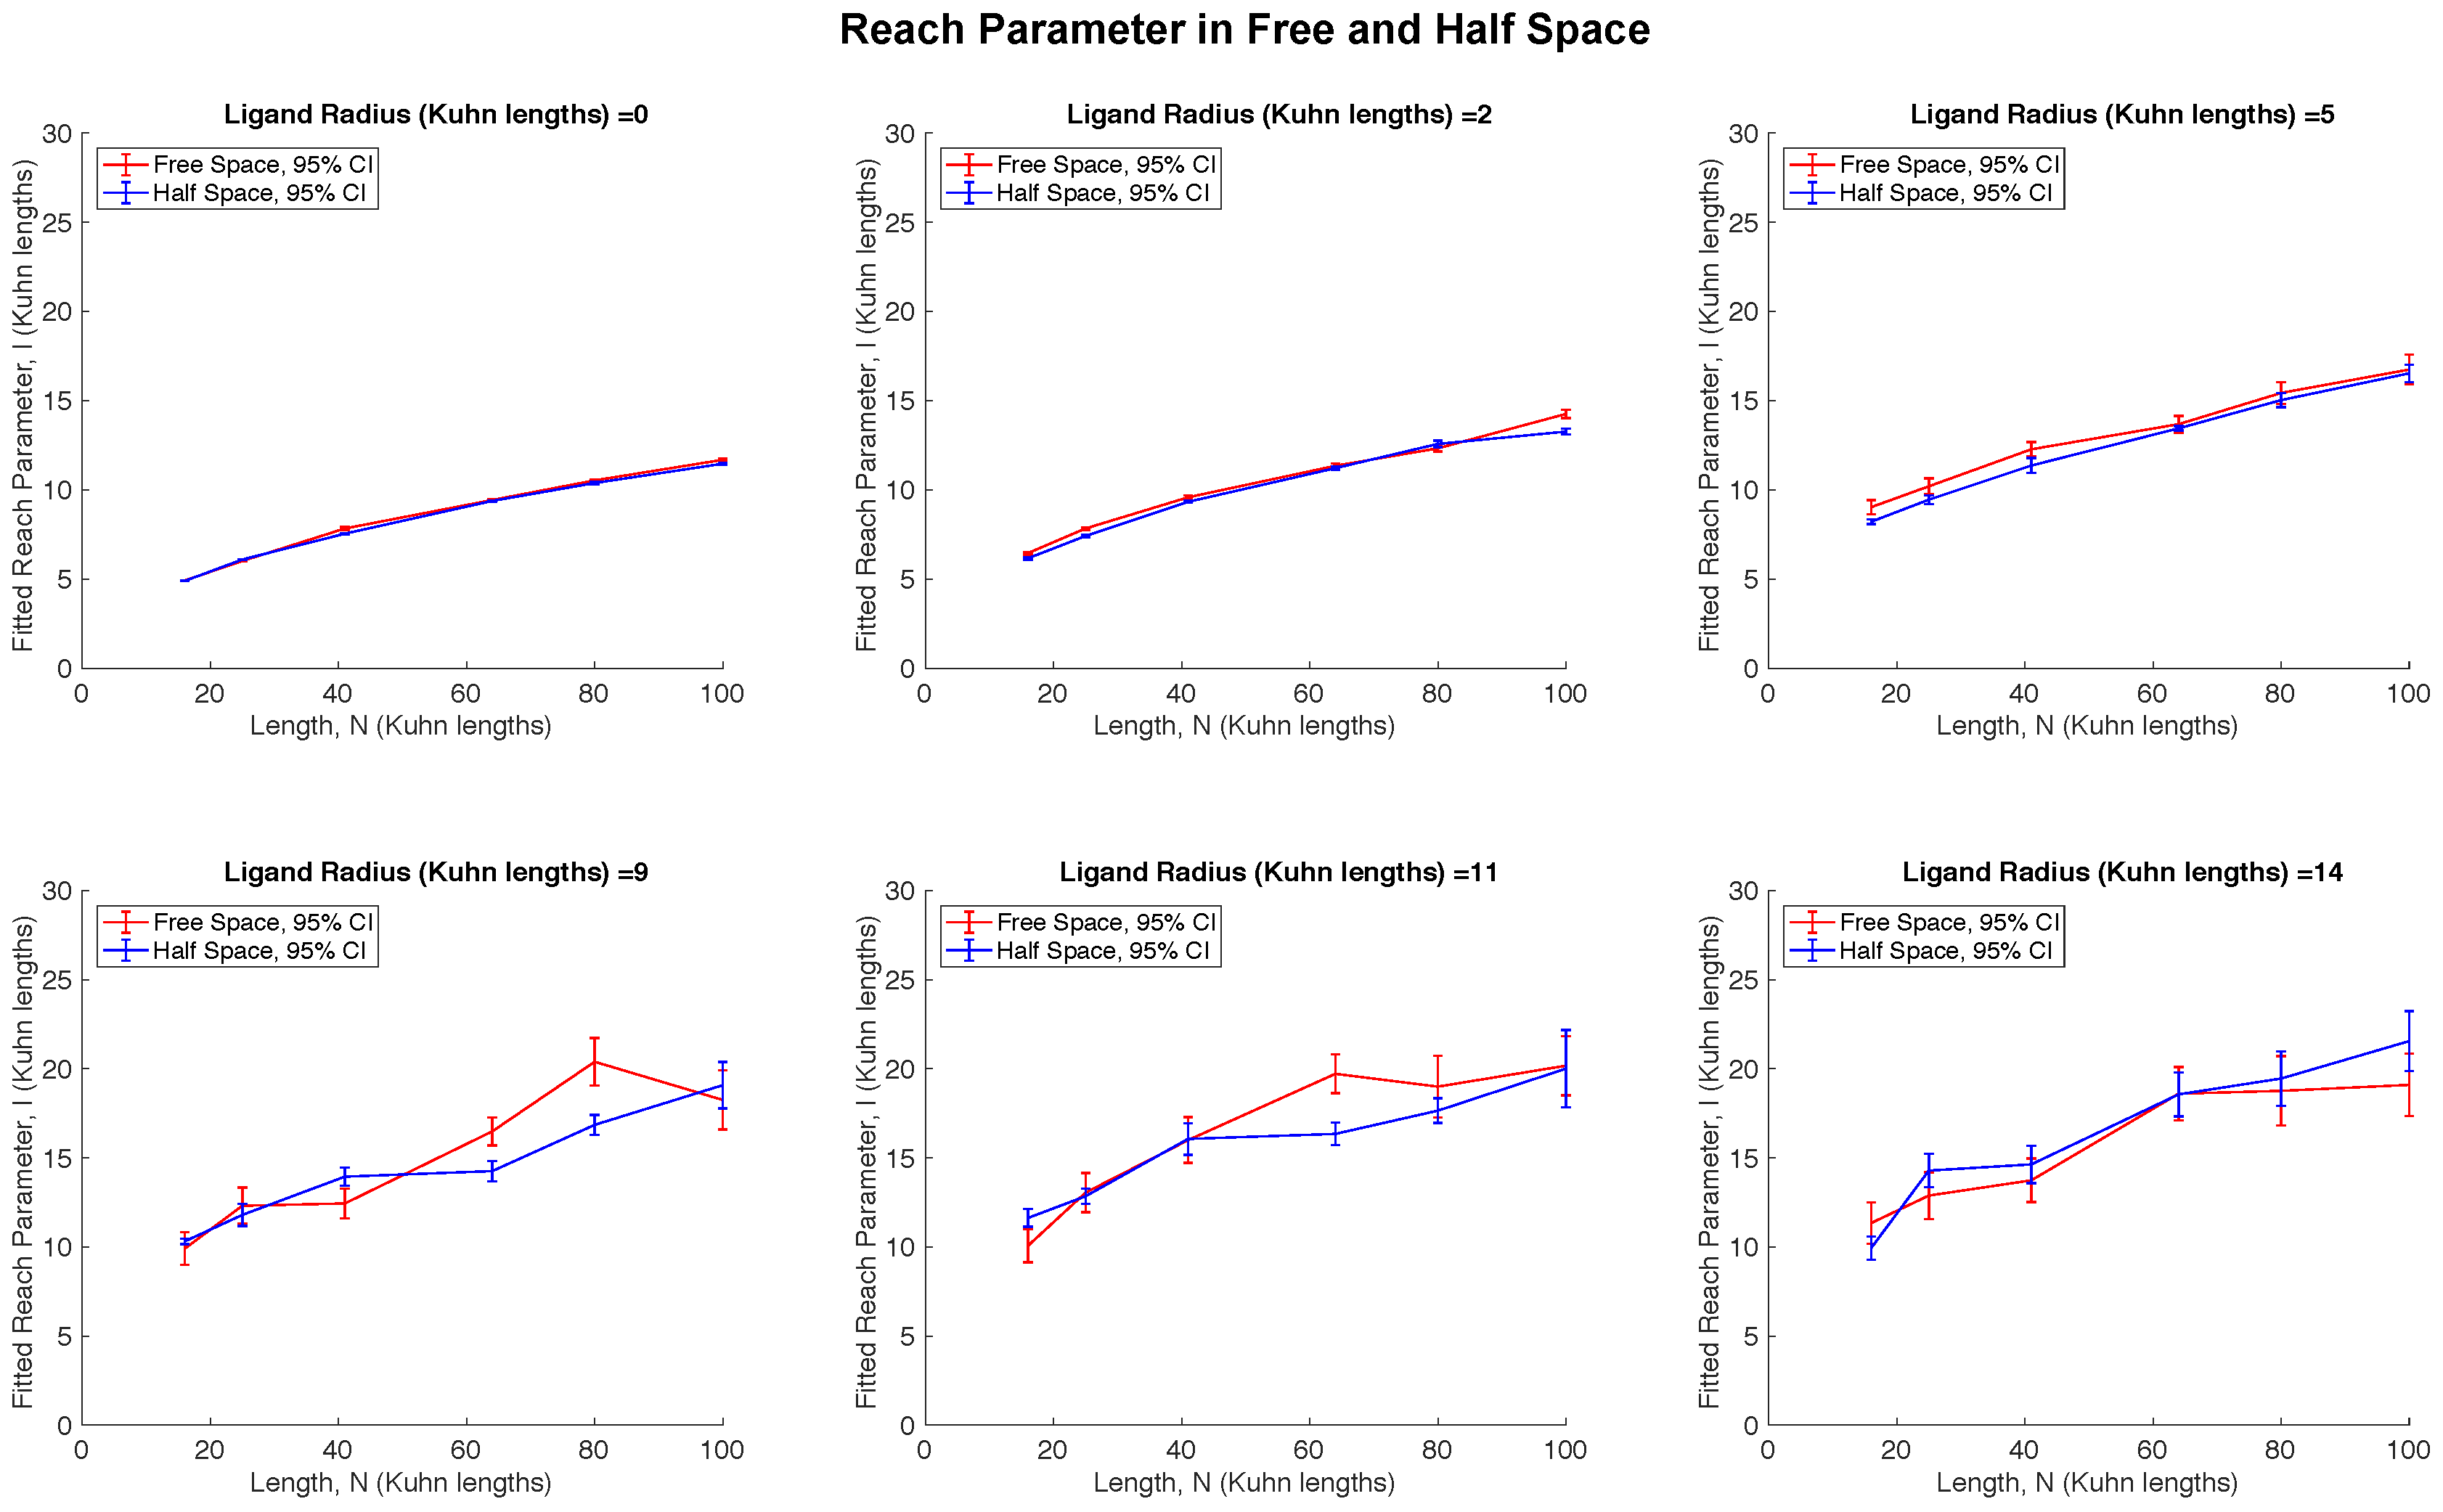
\includegraphics[width=\linewidth]{ResultsFigures/ReachSurfaceFactor/ReachParameterFreeHalfAxisEqual.eps}
%        \caption{Reach parameter of half-gaussian fit to local concentration data plotted as a function of tether length, $N$ for various ligand radii in free-space (red) and half-space (blue) with 95\% confidence intervals for the fit. \label{fig: ReachParameter}}
%    \end{center}
%\end{figure}
%
%\begin{figure}[H]
%    \begin{center}
%        		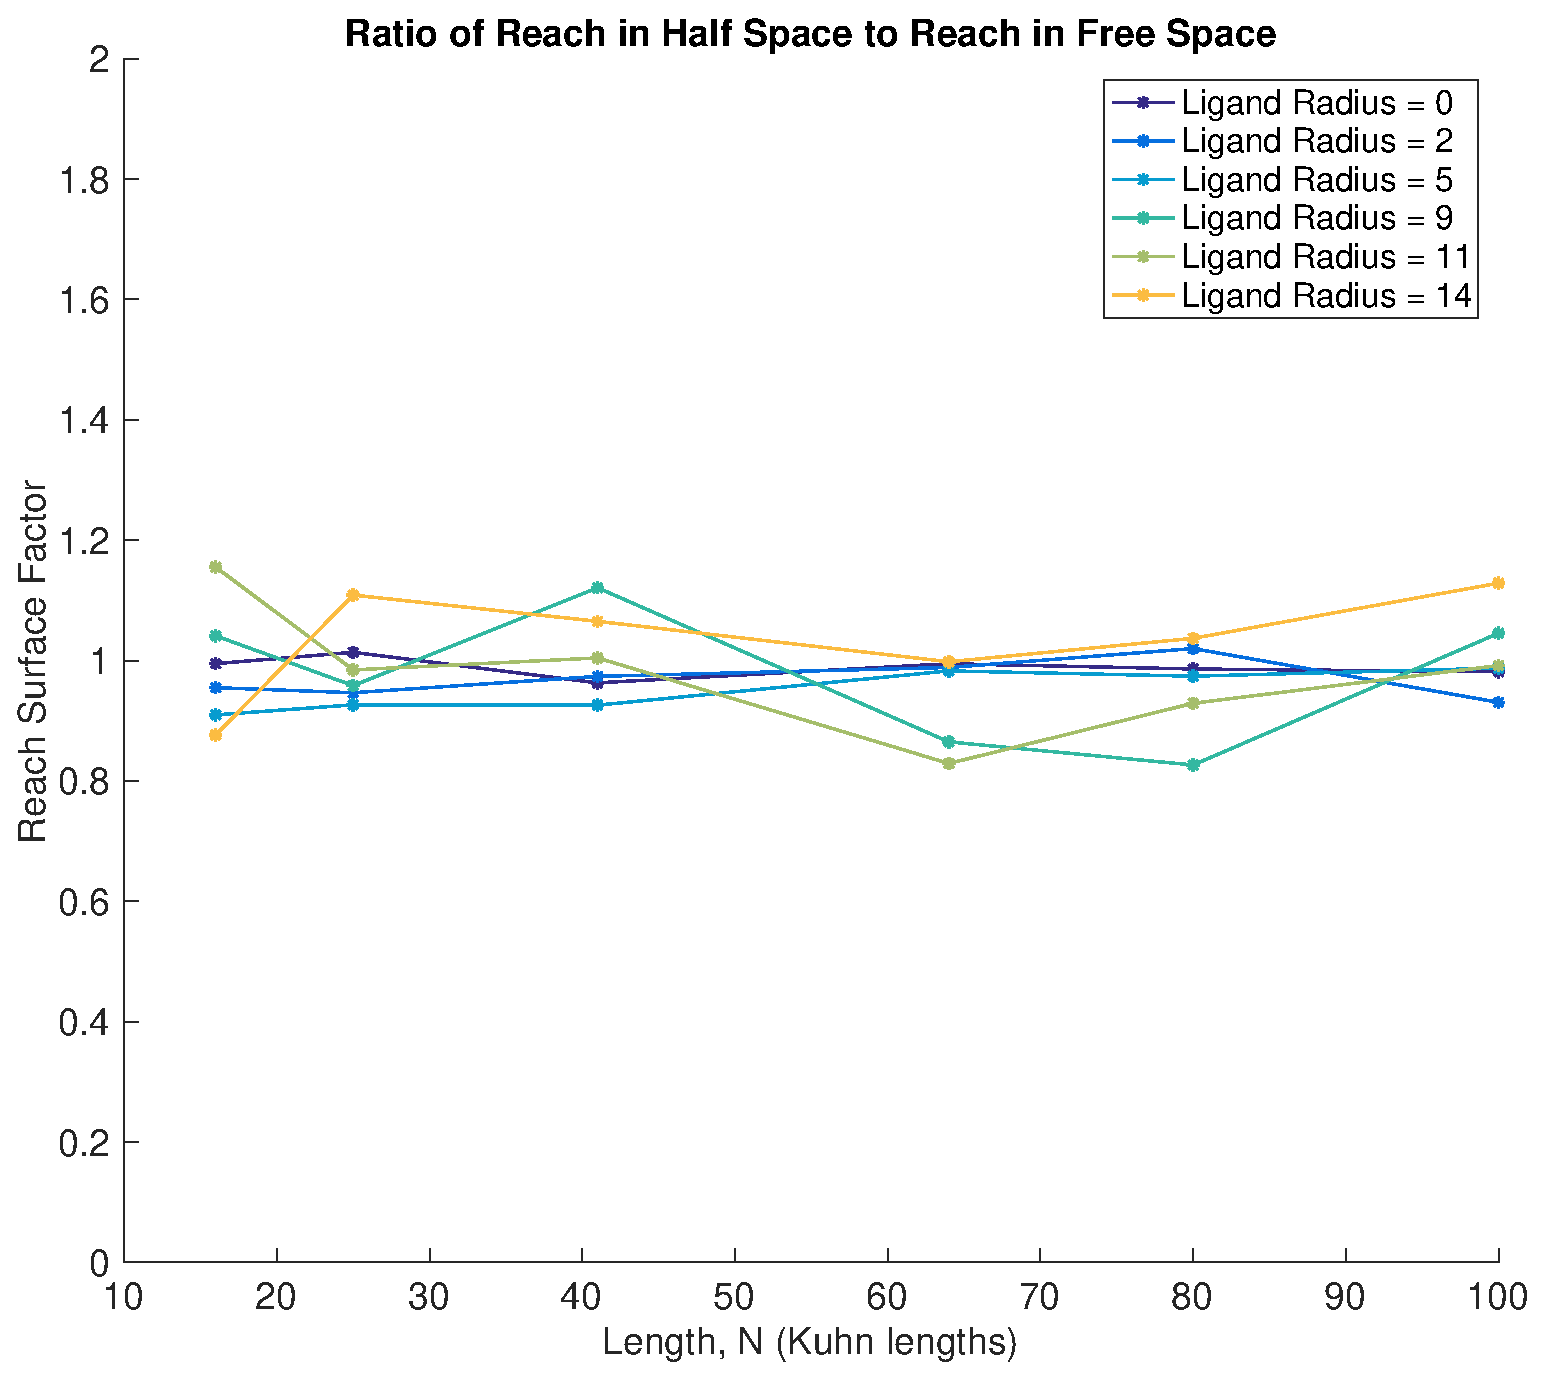
\includegraphics[width=0.7\linewidth]{ResultsFigures/ReachSurfaceFactor/ReachSurfaceFactor.eps}
%        \caption{Ratio of half-space fitted reach parameter to free-space fitted reach parameter as a function of tether length, $N$ (Kuhn lengths), for various ligand radii. \label{fig: ReachSurfaceFactor}}
%    \end{center}
%\end{figure}


\subsubsection{Future Work: Experimental comparison of matrix-bound versus surface-bound tethered reactions}

%Do we need to talk about experimental setup?
% PEG3 K_D increase not 'significant'....

% compare simulation to data
We compare the results from our simulations to preliminary data collected by our collaborators. The data represents the output of surface plasmon resonance experiments conducted with SHP-1 attached to three different tethers (PD1, PEG3, PEG28) on a matrix (CM5) and a surface (C1). 
% We know from first result that since occlusion will show up as K_D, K_D will increase with a membrane.
We found that the presence of a surface will decrease the accessibility of the binding site. This change will cause an increase in the dissociation constant, $K_D$. 
% This matches results
Consistent with our simulated results, the $K_D$ increases when the experiment is conducted on a surface compared to on a matrix for each tether (Fig. \ref{fig: PD1Data}, \ref{fig: PEG3Data}, \ref{fig: PEG28Data}).

% Changes in () will show up as change in k_cat
We will also compare our simulated changes in effective concentration to data. The change in effective concentration will manifest as a change in the observed catalytic rate, $k_{cat}$. 
% We will eventually compare all of this
If we establish a relation between the observed catalytic rate on a surface compared to a matrix, we can recalculate the experimental reach parameter to check for agreement. For example, in the shown data, we assume the observed $k_{cat}$ on a surface is 1.2 fold increased over a matrix (red bar in Fig. \ref{fig: PD1Data}, \ref{fig: PEG3Data}, \ref{fig: PEG28Data}). From this, we can recalculate the reach parameter to compare with simulated results. 




% consider spacing these differently and then creating subfigures
\begin{figure}[h]
	\begin{center}
		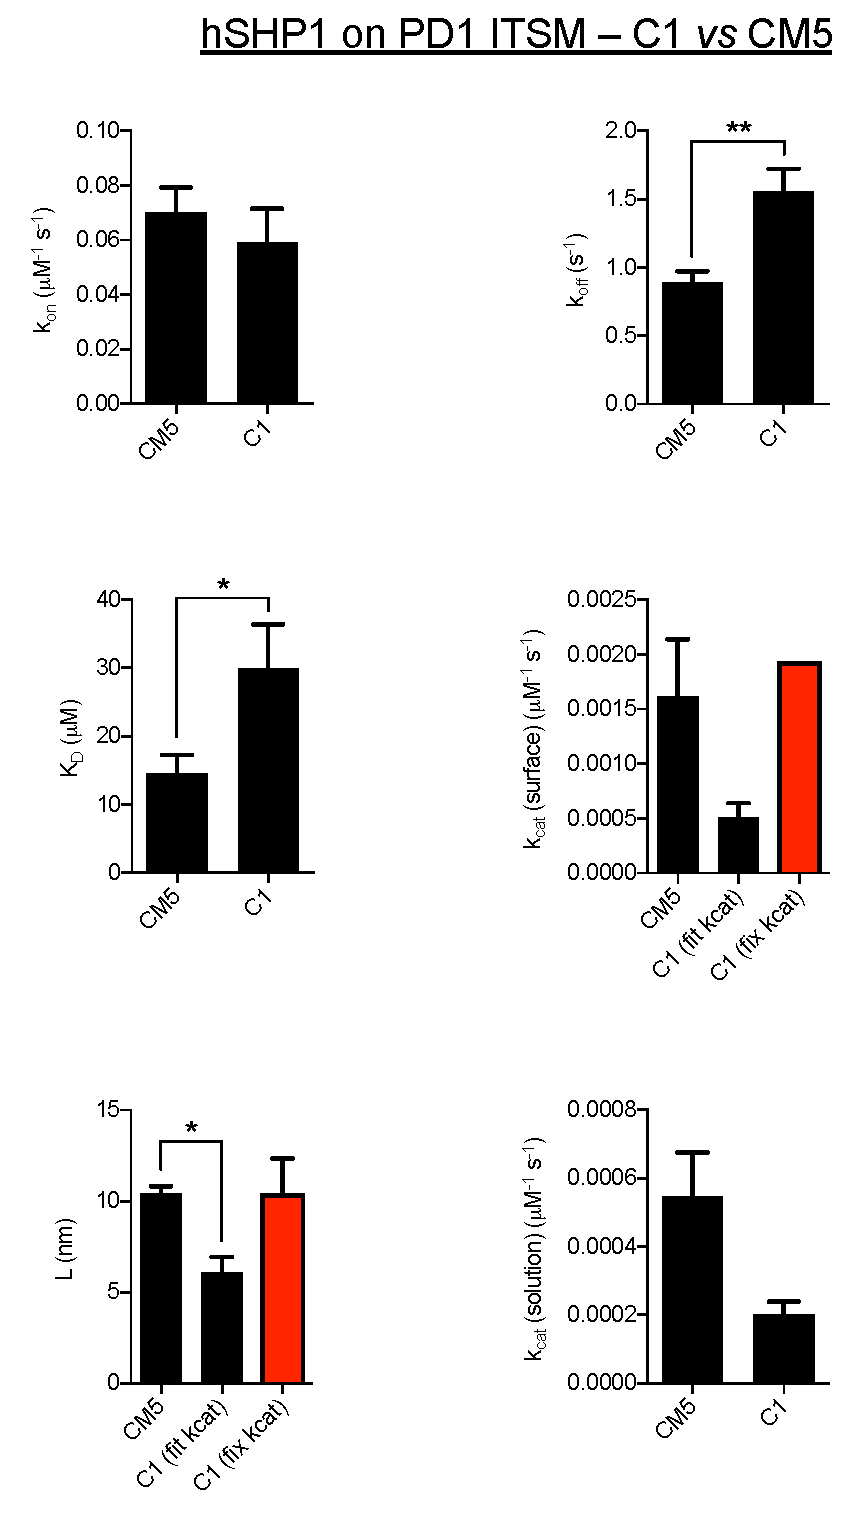
\includegraphics[scale=0.5]{ResultsFigures/ExperimentalDataPlots/hSHP1_on_PD1_ITSM_CM5_vs_C1.pdf}
	\end{center}
	\caption{Preliminary comparison of tethered reaction of human SHP-1 dephosphorylating ITSM on PD1 performed on matrix (CM5) and surface (C1). Comparisons between (a) binding rate, $k_{on}$ (b) unbinding rate, $k_{off}$ (c) dissociation constant, $K_D$ (d) catalytic rate tethered, $k_{cat}$(surface) (e) reach parameter, L, (f) catalytic rate in solution, $k_{cat}$(solution). Change in reach parameter is also calculated under assumption that $k_{cat}$(surface) on a surface is 1.2 fold increased over a matrix (red). \label{fig: PD1Data}}
\end{figure}

\begin{figure}[h]
	\begin{center}
		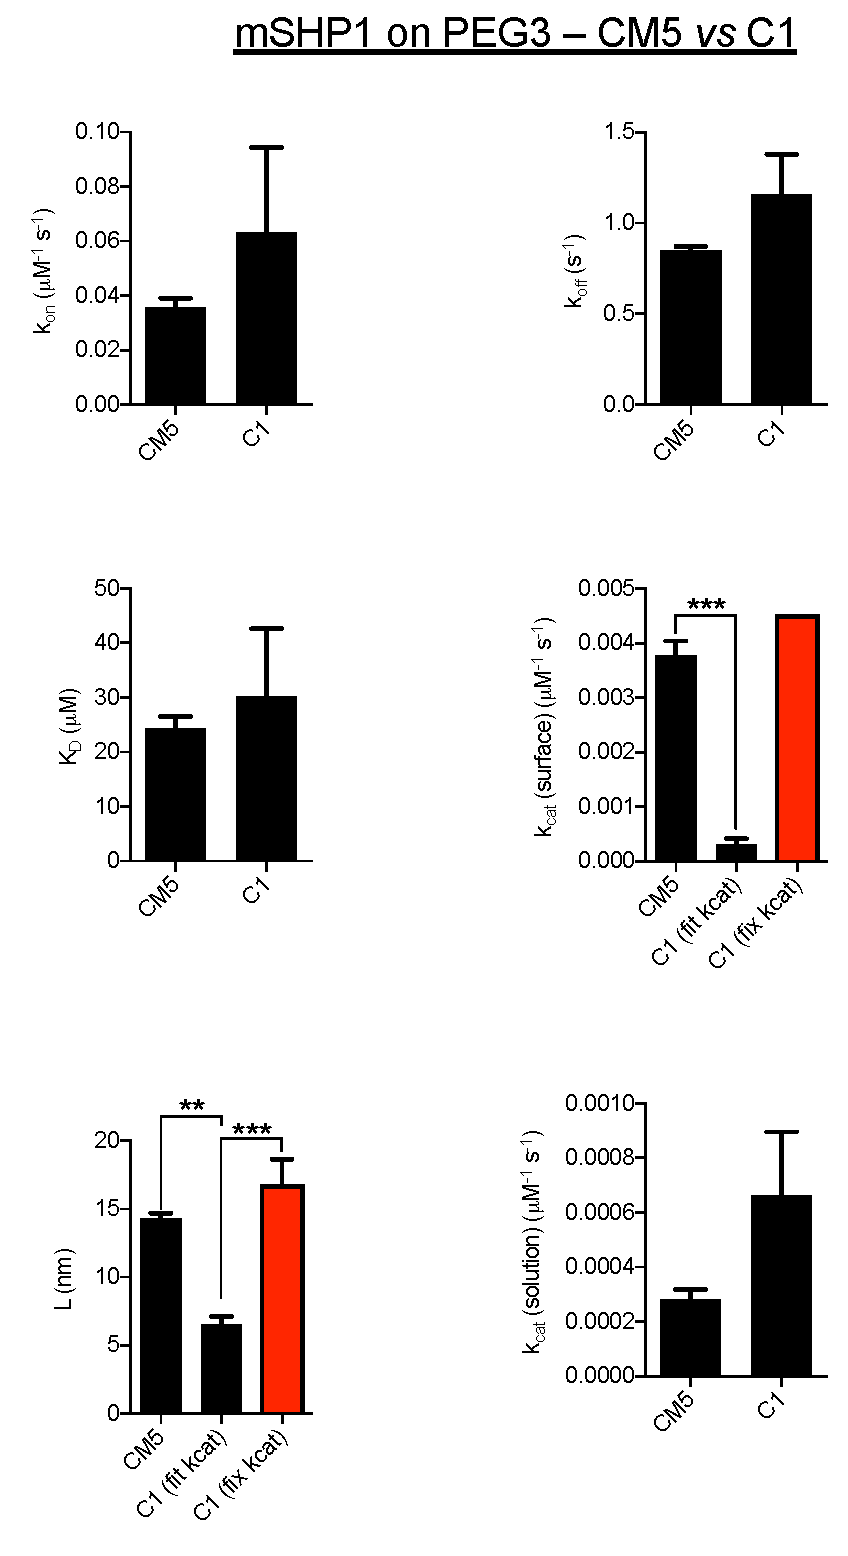
\includegraphics[scale=0.5]{ResultsFigures/ExperimentalDataPlots/mSHP1_on_PEG3_CM5_vs_C1.pdf}. 
	\end{center}
	\caption{Preliminary comparison of tethered reaction of mouse SHP-1 dephosphorylating ITIM on PEG3 performed on matrix (CM5) and surface (C1) assuming tether reach unchanged. Comparisons between (a) binding rate, $k_{on}$ (b) unbinding rate, $k_{off}$ (c) dissociation constant, $K_D$ (d) catalytic rate tethered, $k_{cat}$(surface) (e) reach parameter, L, (f) catalytic rate in solution, $k_{cat}$(solution). \label{fig: PEG3Data}}
\end{figure}

\begin{figure}[h]
	\begin{center}
		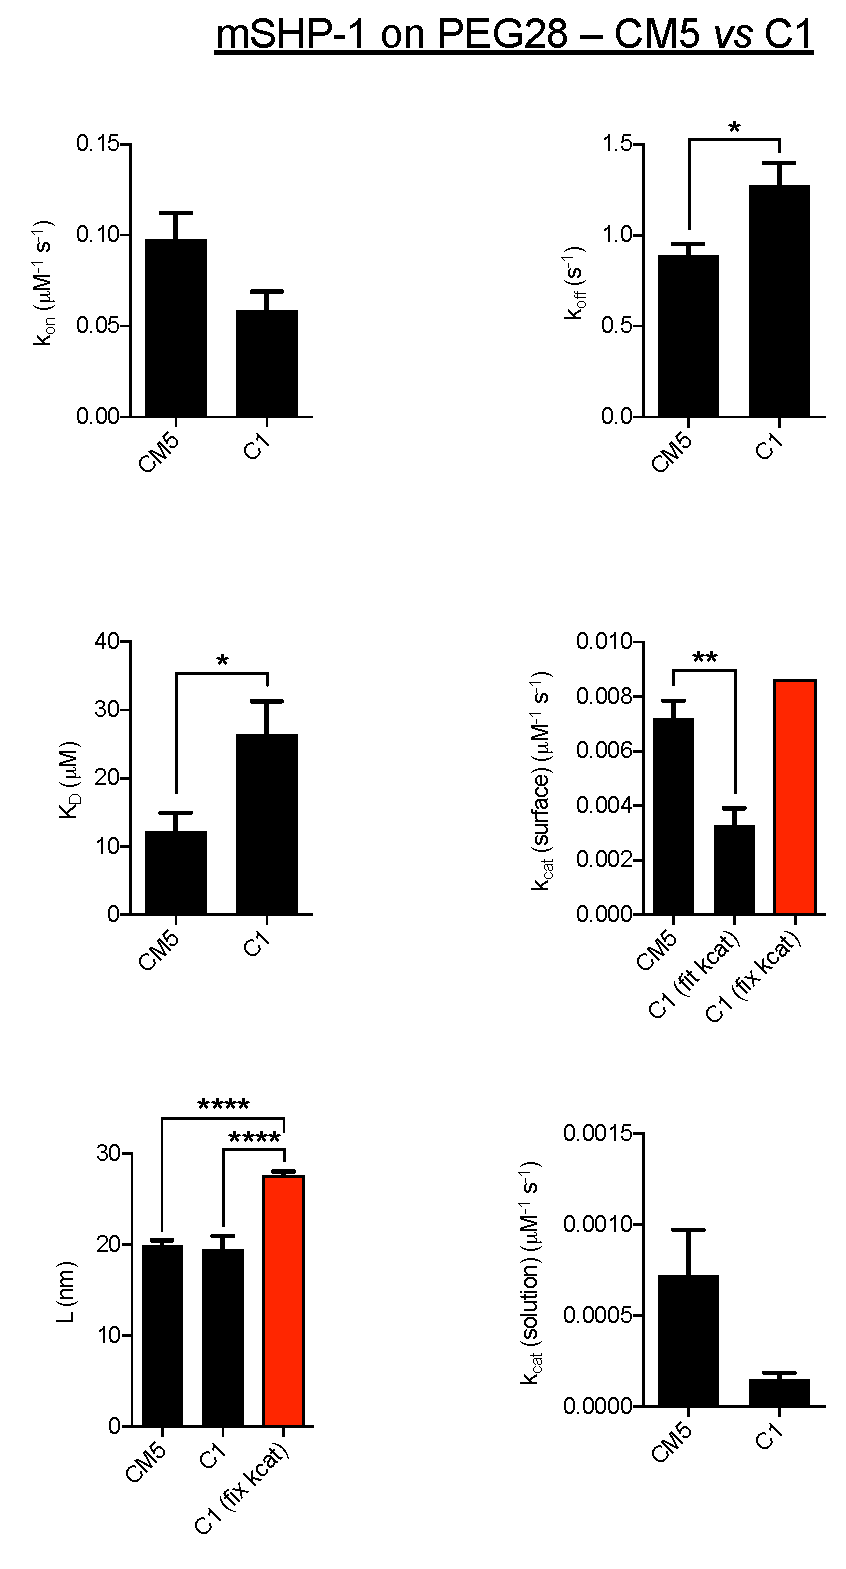
\includegraphics[scale=0.5]{ResultsFigures/ExperimentalDataPlots/mSHP1_on_PEG28_CM5_vs_C1.pdf}
	\end{center}
	\caption{Preliminary comparison of tethered reaction of mouse SHP-1 dephosphorylating ITIM on PEG28 performed on matrix (CM5) and surface (C1) assuming tether reach unchanged. Comparisons between (a) binding rate, $k_{on}$ (b) unbinding rate, $k_{off}$ (c) dissociation constant, $K_D$ (d) catalytic rate tethered, $k_{cat}$(surface) (e) reach parameter, L, (f) catalytic rate in solution, $k_{cat}$(solution).\label{fig: PEG28Data}}
\end{figure}


%\begin{figure}[h]
%\begin{center}
%\begin{subfigure}{0.3\linewidth}
%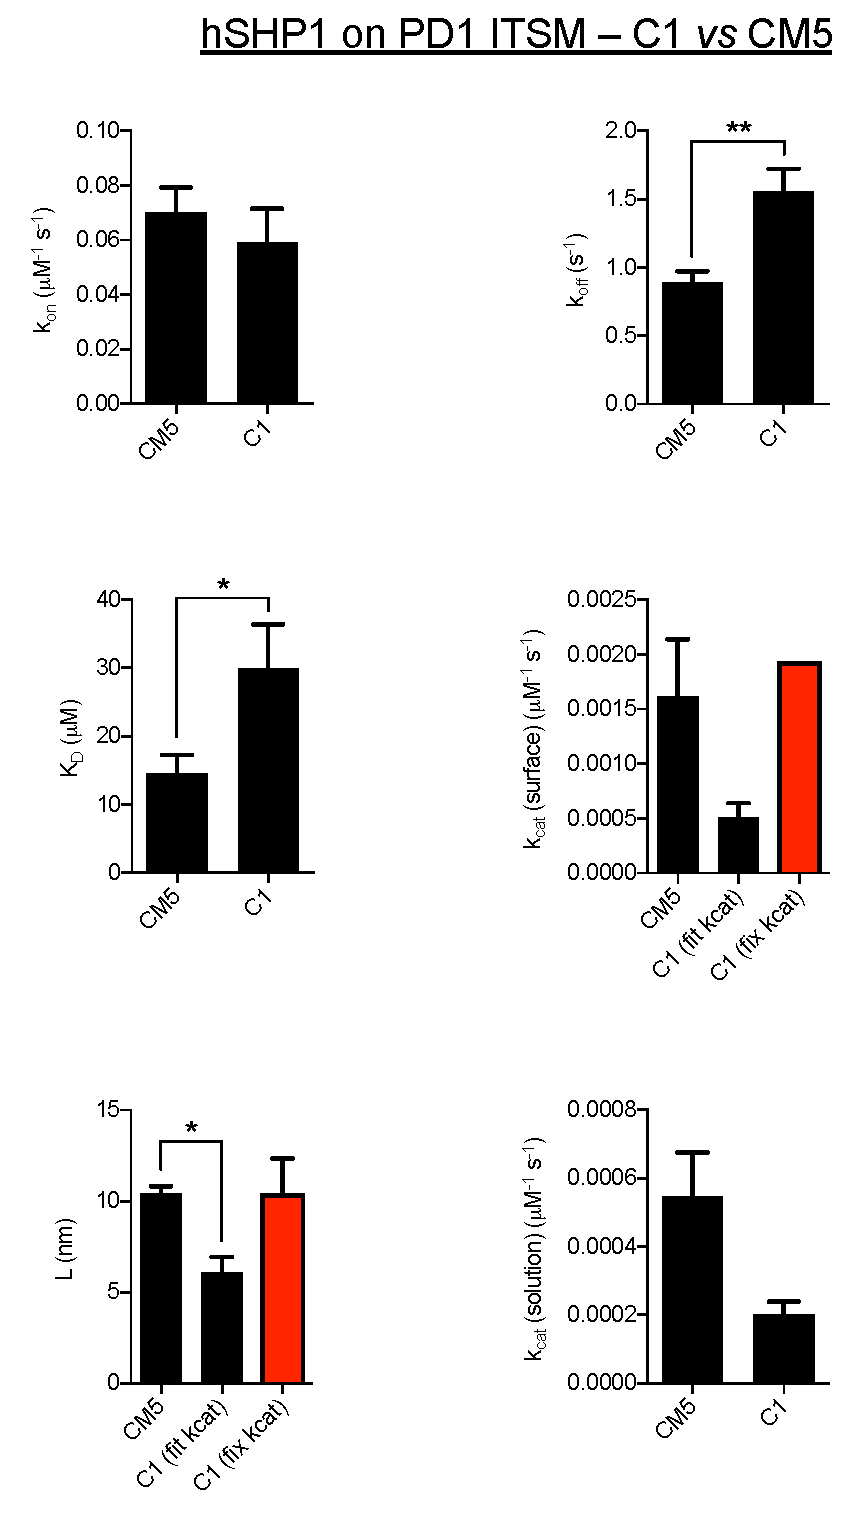
\includegraphics[width=\linewidth]{ResultsFigures/ExperimentalDataPlots/hSHP1_on_PD1_ITSM_CM5_vs_C1.pdf}
%\caption{}
%\end{subfigure}
%\begin{subfigure}{0.3\linewidth}
%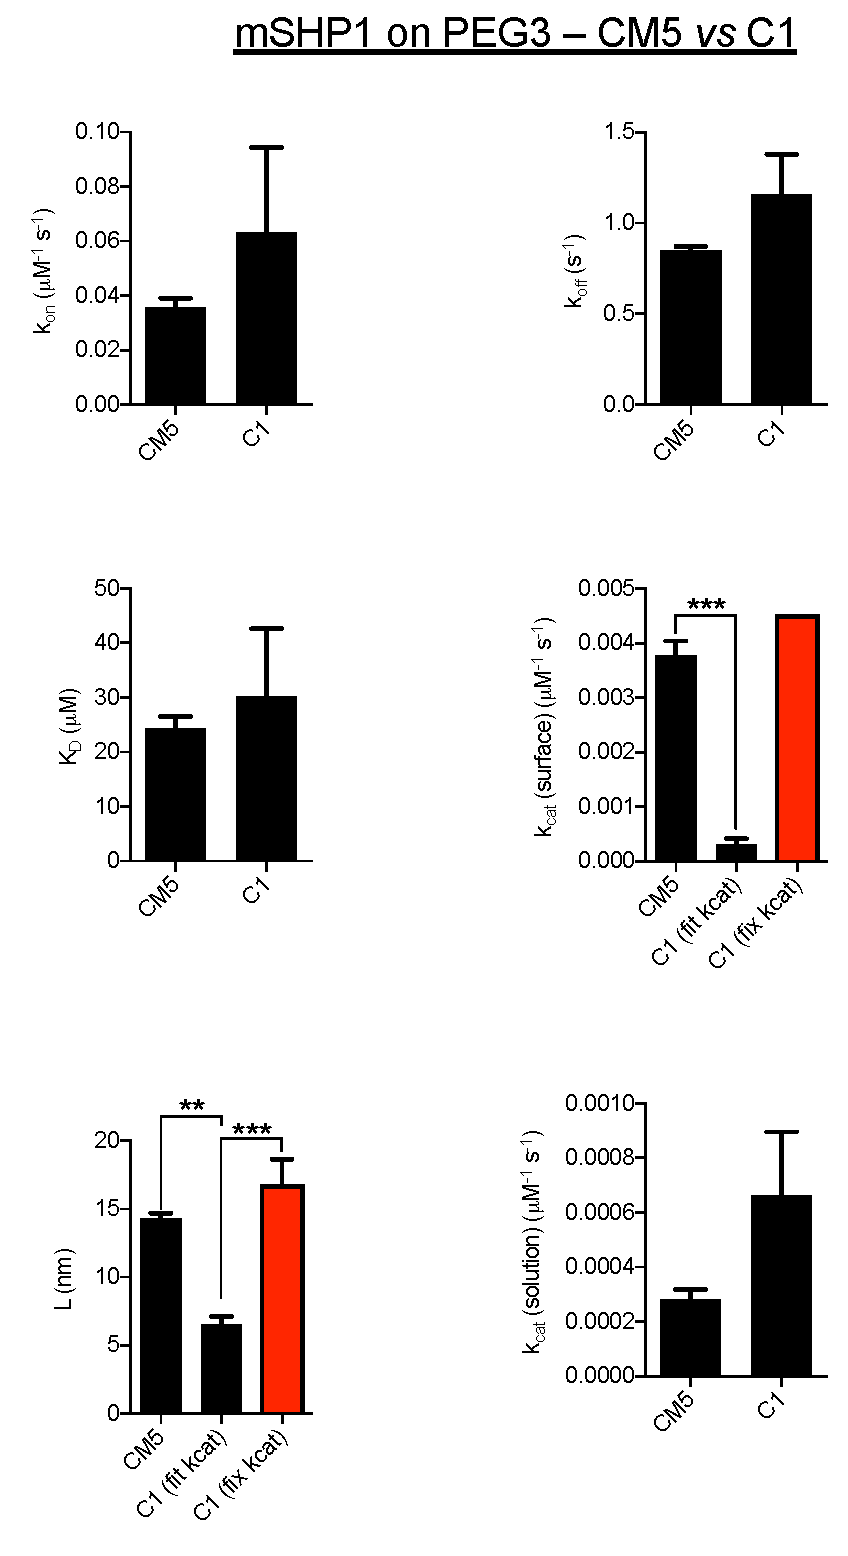
\includegraphics[width=\linewidth]{ResultsFigures/ExperimentalDataPlots/mSHP1_on_PEG3_CM5_vs_C1.pdf}
%\caption{}
%\end{subfigure}
%\begin{subfigure}{0.3\linewidth}
%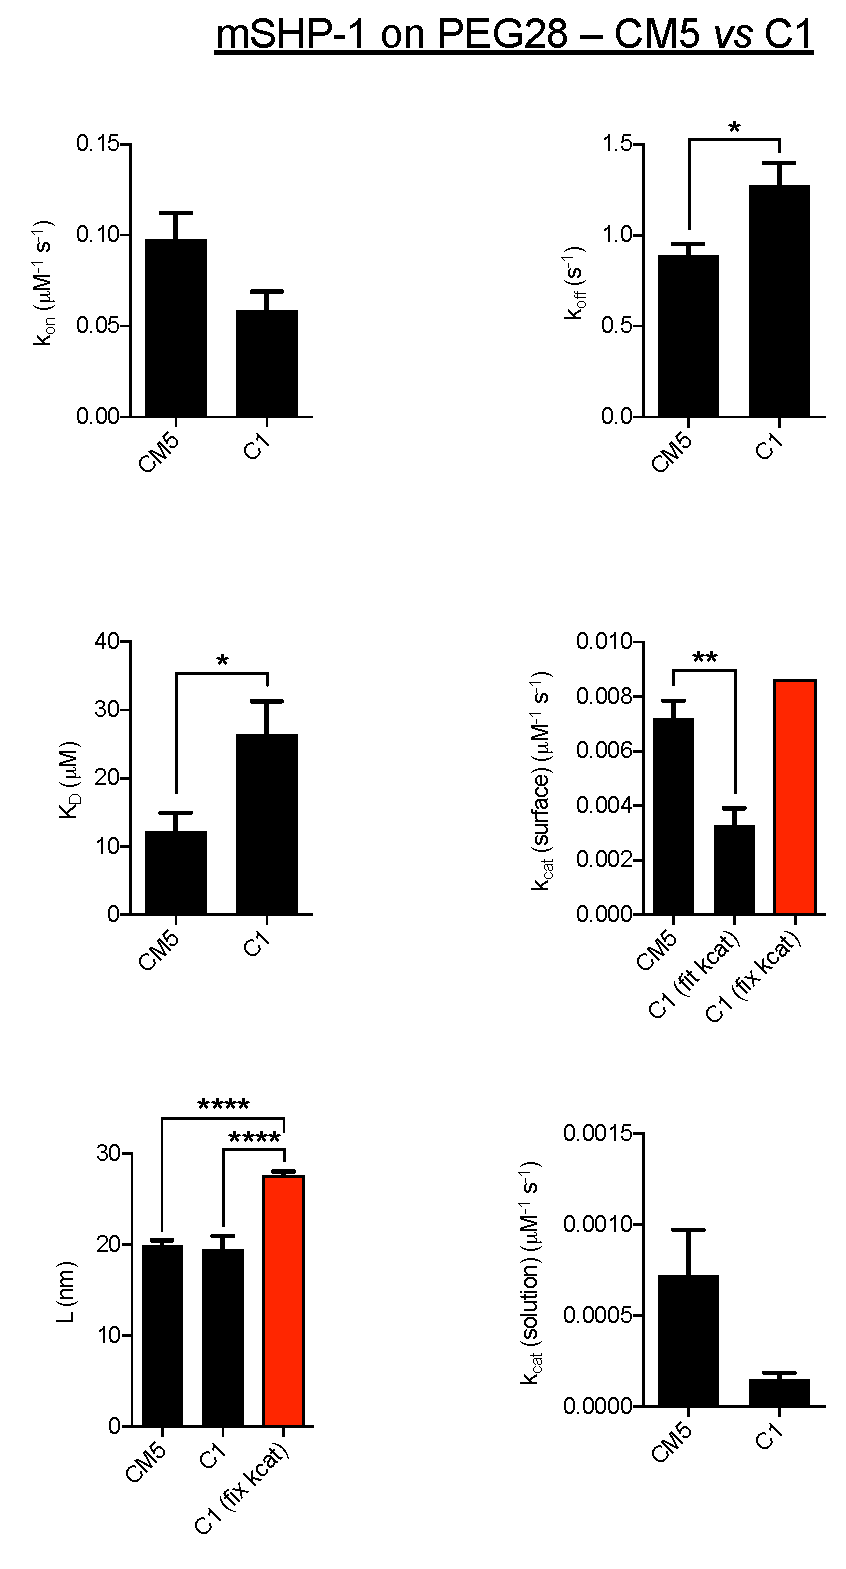
\includegraphics[width=\linewidth]{ResultsFigures/ExperimentalDataPlots/mSHP1_on_PEG28_CM5_vs_C1.pdf}
%\caption{}
%\end{subfigure}
%\end{center}
%\end{figure}



\subsubsection{Future Work: Catalysis surface factor $\kappa^{(teth2teth)}_{cat}$ versus $l_C$ and/or versus $r_{ligand}$}

Experimental measurements of effective concentration do not distinguish between the effective concentration and the catalytic rate. Since these values are lumped into a single number, it is important to know how the surface impacts the apparent catalytic rate. We will plot the ratio of apparent catalytic rates for various polymer lengths and ligand sizes. This will indicate if there is a relationship between the catalysis factor and the reaction parameters or if there is a single value describing the impact of the surface. The catalysis surface factor may then be used to determine how experiments on a surface differ from on a matrix and possibly give a conversion factor between the two. 










%%%%%%%%%%%%%%%%%%%%%%%%%%%%%%%%%%%%%%%%%%%%%%%%%%%
\end{document}
%%%%%%%%%%%%%%%%%%%%%%%%%%%%%%%%%%%%%%%%%%%%%%%%%%%





